\chapter{Umsetzung}
\label{chap:data_collection}
F{\"u}r die Umsetzung wurden die in Abbildung \ref{fig:inhalt_semesterarbeit}, Inhalt der Semesterarbeit, dargestellten Arbeitsschritte durchgef{\"u}hrt:

\begin{itemize}
  \item Auswahl zu verwendenden Docker Images / Container  
  \item Erstellen der docker-compose Datei
  \item Anpassung der detect-hate App um Tweets zu klassifizieren 
  \item Softwarekomponenten konfigurieren
  \item Pipelines in StreamSets erstellen
  \item Kibana Dashboard erstellen
  \item On-Prem Bigboards Cluster (nHex) konfigurieren (Kubernetes Setup \& Konfiguration)
  \item Streaming und Analyseumgebung auf den nHex Cluster portieren
\end{itemize}

Diese Schritte werden in diesem Kapitel detailliert erkl{\"a}rt. Bez{\"u}glich  Vorgehen l{\"a}sst sich noch erg{\"a}nzend sagen, dass die Umsetzung bewusst iterativ erfolgt. Die Datenbanken, Indexes, und das Dashboard haben einen Einfluss auf die einzelnen Schritte in der Pipeline, welche erste im Laufe der Arbeit festgestellt werden k{\"o}nnen und eine wiederum eine Anpassung der einzelnen vorangehenden Schritte in den Pipelines nach sich zieht.

Wie im Kapitel \ref{sec:introduction_solution} L{\"o}sungsansatz beschrieben wird die L{\"o}sung zuerst lokal auf dem Macbook  entwickelt und  anschliessend auf den nHex portiert. Dies hat den Hintergrund, dass es leichter ist die Anwendung lokal, mittels docker-compose auf einem Rechner zu entwickeln und 'produktionsreif' zu bringen, als direkt auf einem Big Data Cluster mit Kubernetes und sechs Nodes. 

\section{Architektur}
\label{sec:rchitecture}
Die Architektur der Streaming und Analyse Umgebung besteht aus den in Kapitel \ref{sec:streaming} beschriebenen Komponenten und ist gezielt modular gestaltet: 

\begin{itemize}
  \item Docker: Einzelne Software Komponenten
  \item Streamsets: Bau der Pipelines f{\"u}r ETL/ELT
  \item Kafka: Verteilen und Zwischenspeichern der Nachichten zwichen den Komponenten
  \item MongoDB: Rohdaten von Twitter f{\"u}r die Masterarbeit speichern
  \item Elasticsearch: Bearbeitete Daten von Twitter und Klassifikation speichern
  \item Kibana: Dashboard f{\"u}r Analyse visualiseren
\end{itemize}

Die modulare Gestaltung hat den Vorteil, dass diese Architektur die Anwendung robuster und leichter erweiterbar macht. In Abbildung \ref{fig:local_high_level_architecure} sind die Architektur mit den verwendeten Komponenten und der Kommunikationsfluss dargestellt. F{\"u}r jede Softwarekomponente wurde ein separater Dockercontainer erstellt, so dass {\"A}nderungen an den einzelnen Konfigurationen ohne Einfluss auf andere Komponenten vorgenommen werden k{\"o}nnen.

\begin{figure}[H]
	\centering
		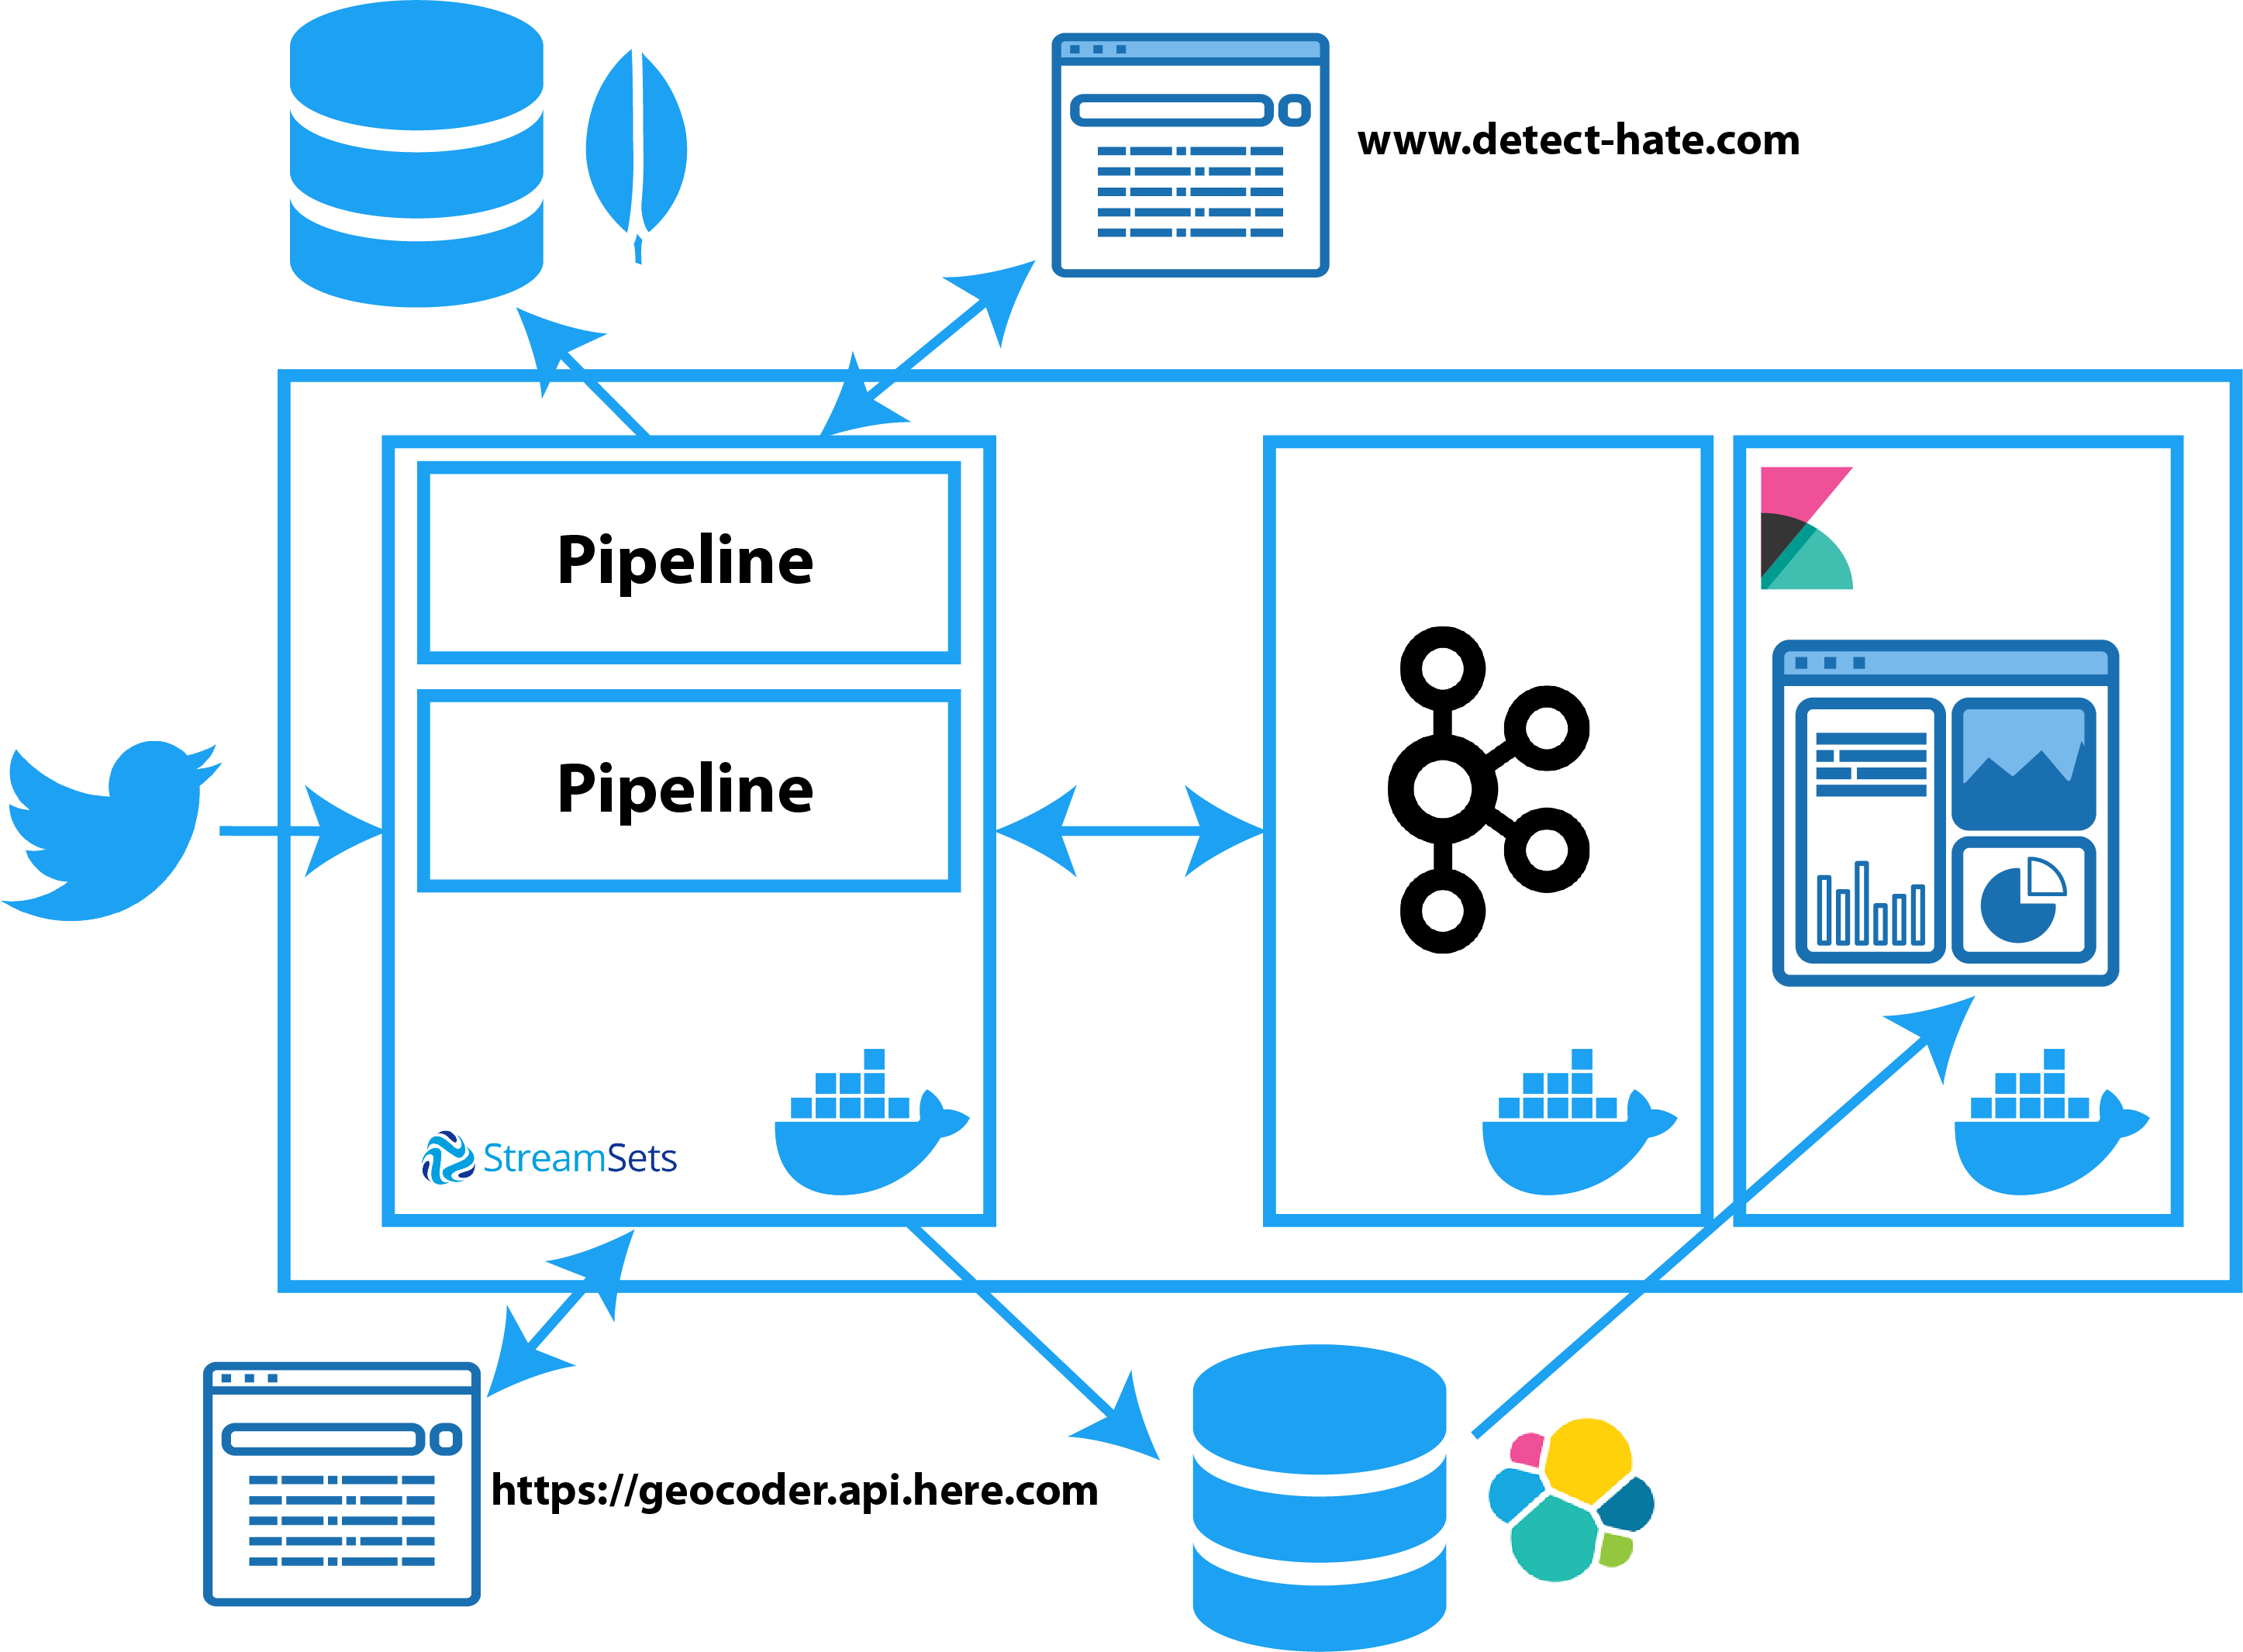
\includegraphics[scale=0.4 ]{images/architecktur_high_level.png}
	\caption{Architektur lokal}
	\label{fig:local_high_level_architecure}
\end{figure}

Abbildung \ref{fig:architecture_nhex} zeigt die Architektur auf dem nHex Big Data Cluster. Die Architektur ist komplexer wie lokal, da der nHex 6 Nodes hat. Auch hier wurde auf eine saubere Kapselung und Trennung der Servcies wert gelegt. In Kapitel \ref{sec:nHex} sind die zur Implementation n{\"o}tigen Schritte beschrieben. 

\begin{figure}[H]
	\centering
		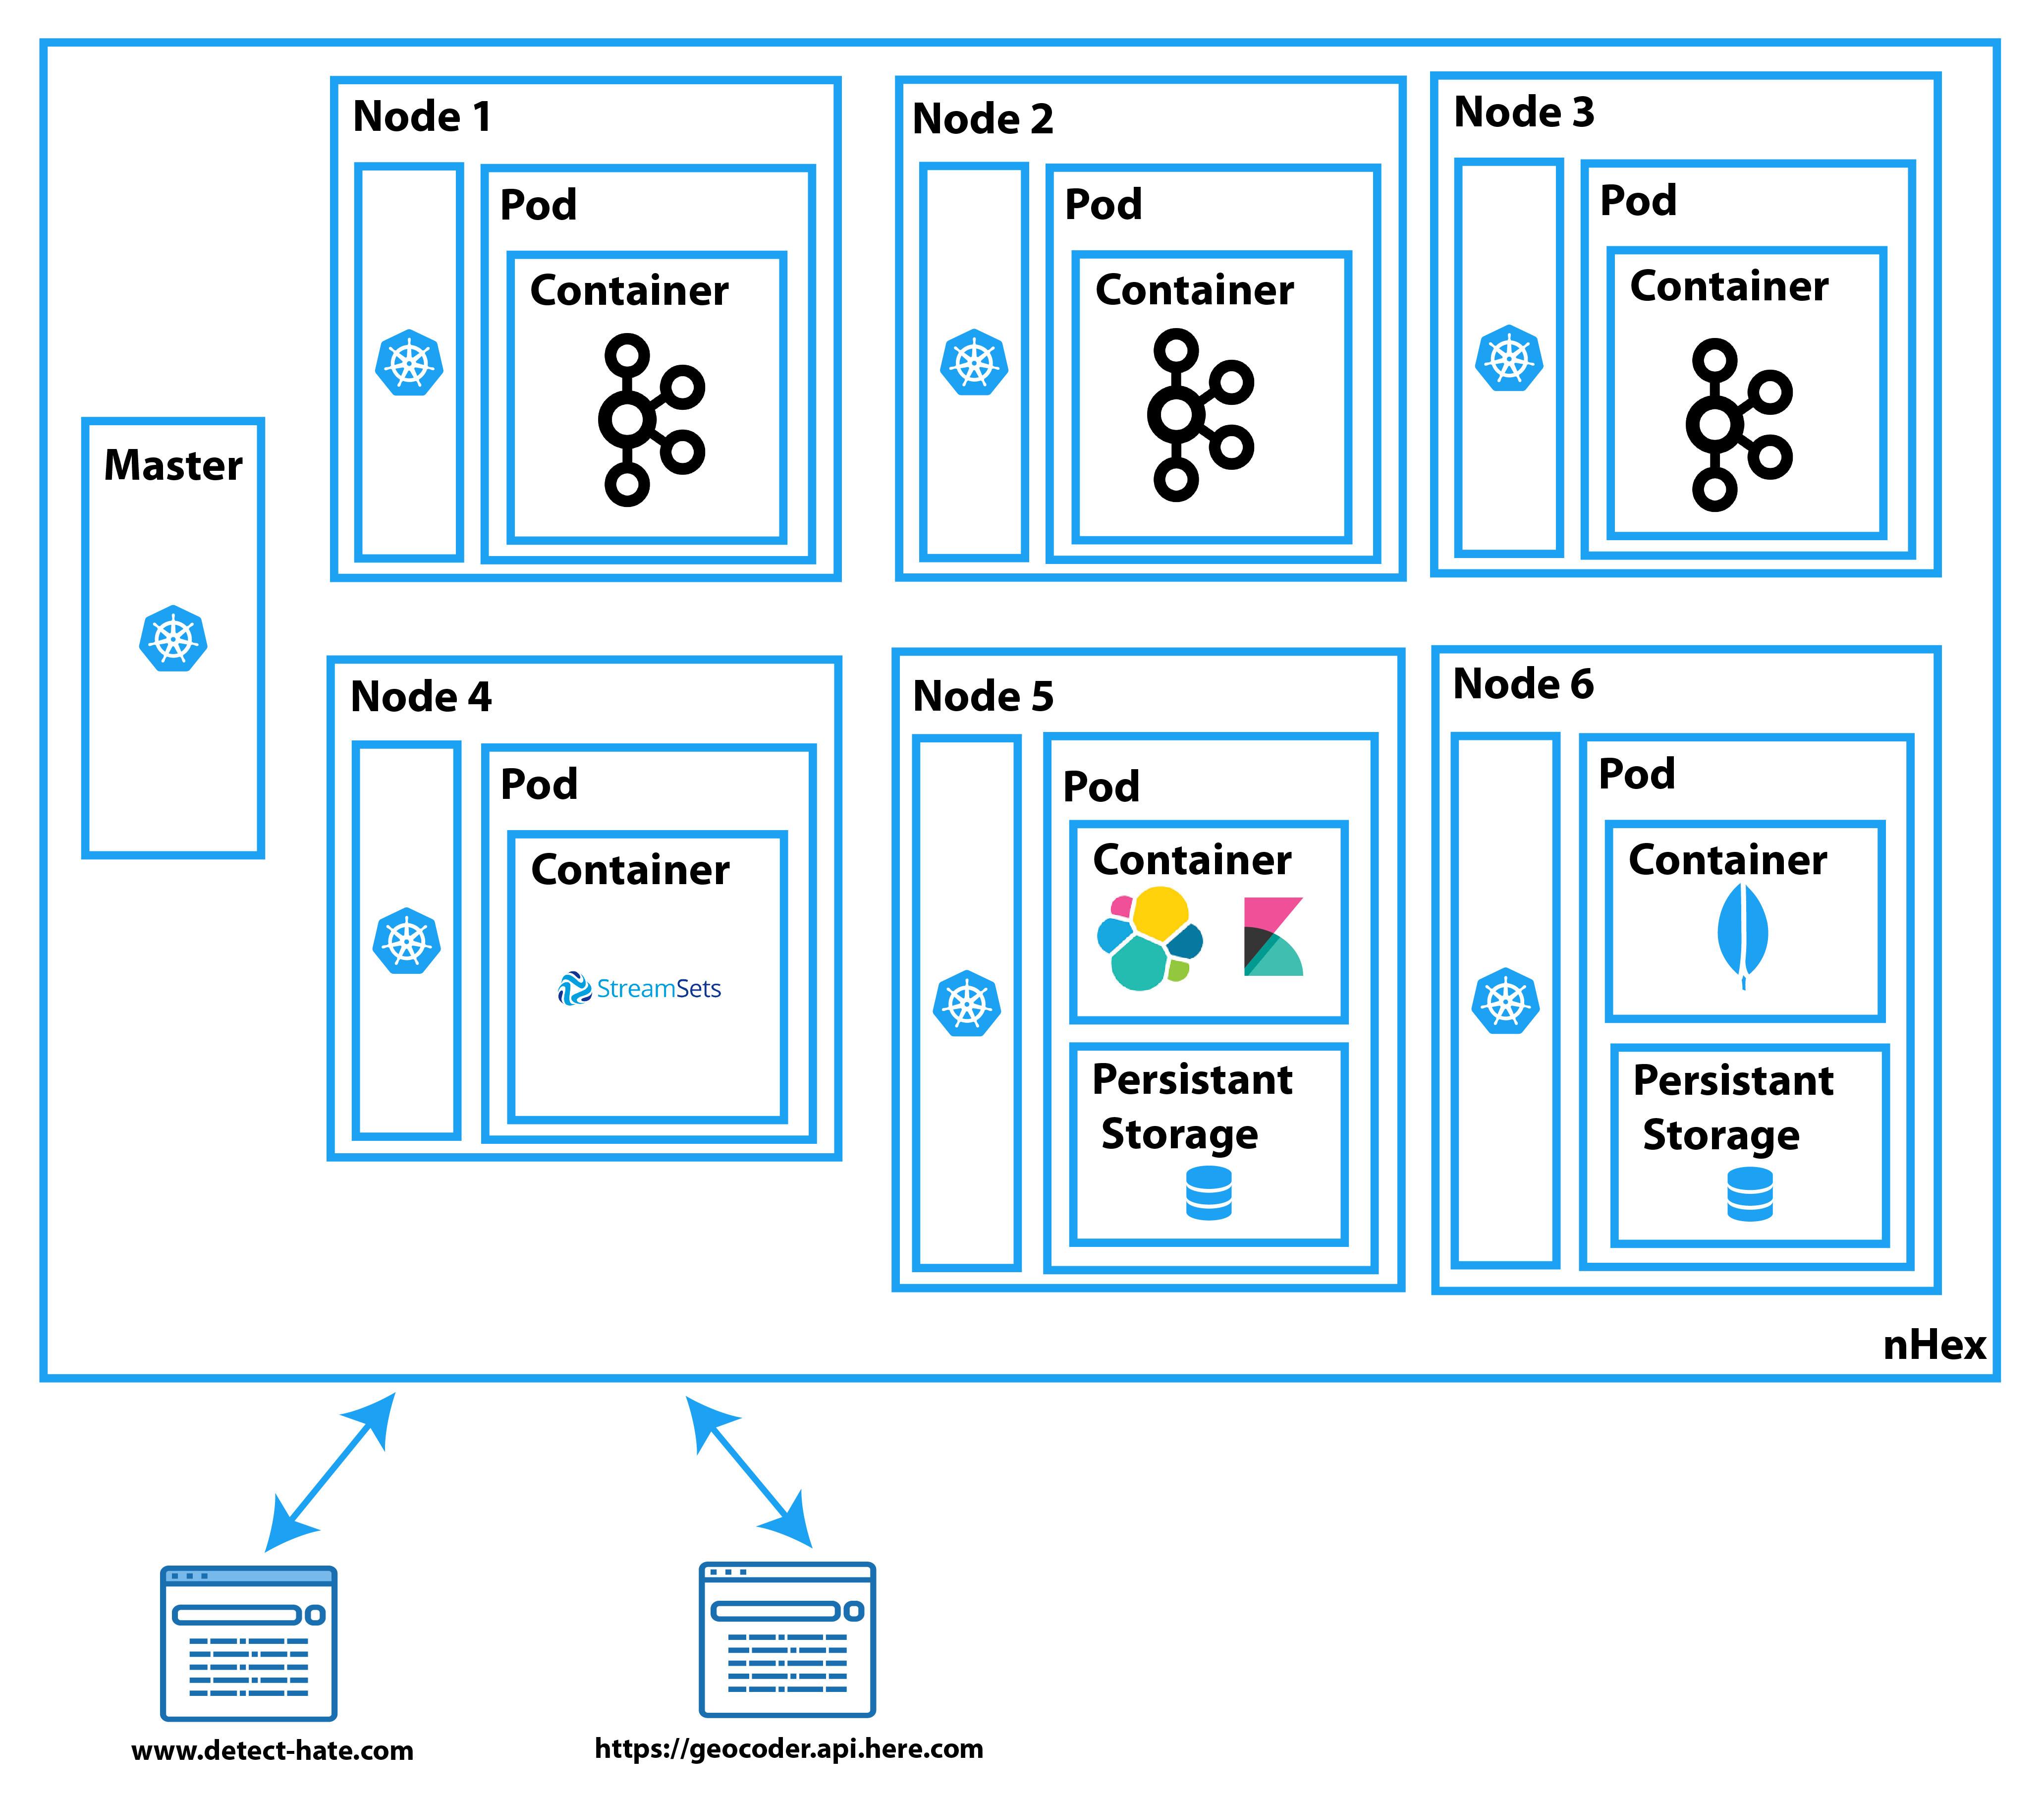
\includegraphics[scale=0.4 ]{images/architecktur_high_level_nhex-02-02.png}
	\caption{Architektur nHex}
	\label{fig:architecture_nhex}
\end{figure}

\section{Aufbau docker-compose.yml }
\label{sec:docker_compose}

Die docker-compose Datei beinhaltet alle verwendeten Software Komponenten (Container \& Services) und die n{\"o}tigen Konfigurationen inklusive Dependecies. In dem folgenden Codeauszug \ref{lst: docker-compose.yml} ist der Aufbau der docker-compose.yml Datei beschrieben. Das vollst{\"a}ndige docker-compse.yml dieser Semesterarbeit ist in \href{https://github.com/verenamai/bgd_term}{Github} abgelegt, da es um einiges gr{\"o}sser, komplexer ist und aus knapp 300 Zielen besteht.
  
\begin{lstlisting}[basicstyle=\tiny,float=h,language=bash,frame=tb,caption={Aufbau docker-compose.yml},label=lst: docker-compose.yml]
version: '3'
services:
	#broker-1
	broker-1: 
		image: confluentinc/cp-kafka:5.2.1
		container_name: broker-1
		hostname: broker-1
		depends_on:
			- zookeeper-1
		ports:
			- "9092:9092"
		environment:
			KAFKA_BROKER_ID: 1
			KAFKA_BROKER_RACK: 'r1'
			KAFKA_ZOOKEEPER_CONNECT: 'zookeeper-1:2181'
			KAFKA_ADVERTISED_LISTENERS: 'PLAINTEXT://${DOCKER_HOST_IP}:9092'
			KAFKA_OFFSETS_TOPIC_REPLICATION_FACTOR: 3
			KAFKA_GROUP_INITIAL_REBALANCE_DELAY_MS: 0
			KAFKA_DELETE_TOPIC_ENABLE: 'true'
			KAFKA_AUTO_CREATE_TOPICS_ENABLE: 'false'
			KAFKA_JMX_PORT: 9994
			KAFKA_JMX_OPTS: '-Dcom.sun.management.jmxremote -Dcom.sun.management.jmxremote.authenticate=false \
			  -Dcom.sun.management.jmxremote.ssl=false -Dcom.sun.management.jmxremote.local.only=false \
			  -Dcom.sun.management.jmxremote.rmi.port=9994'
			KAFKA_JMX_HOSTNAME: 'broker-1'
    				restart: always
    				
    #broker-2		
		 .......
		 .......
volumes:
	 mongodb:
	   external: true

\end{lstlisting}  

Eine docker-compose Datei ist in vier syntaktisch Bereiche eingeteilt, siehe Tabelle \ref{tab:datei_syntax}.

\begin{table}[H]
	\centering
		\begin{tabular}{c|p{12cm}}
		\hline
			version & Gibt die Syntaxversion der Compose Datei an. In dieser Arbeit wird mit Version 3 gearbeitet. \\ \midrule
			services  & Der Name f{\"u}r einen "Container in Produktion". In diesem Abschnitt werden die zu verwendenden
			Container festgelegt,welche als Teil der Docker Compose Instanz gestartet werden. \\ \midrule
			networks & Dieser Abschnitt wird verwendet, um das Netzwerk f{\"u}r die Anwendung zu konfigurieren. (kommt im obigen Beispiel nicht vor.) \\ \midrule
			volumes & Pfad auf den Hostcompter um Daten ausserhalb des Containers zu speichern.\\ \bottomrule
		\end{tabular}
	\caption{Syntax docker-compose.yml}
	\label{tab:datei_syntax}
\end{table}

In der Tabelle \ref{tab:services} sind die m{\"o}glichen Konfigurationsparameter f{\"u}r einen Service beschrieben.

\begin{table}[H]
	\centering
		\begin{tabular}{c|p{12cm}}
			image & Legt das Image fest, welches zum Erstellen des Containers verwendet wird. Das angegebene Image muss 
			entweder auf dem Host oder auf  \href{https://hub.docker.com}{Docker Hub} existieren. \\ \midrule
			build & Dieser Parameter kann anstelle von image verwendet werden und gibt den Speicherort der Dockerdatei an,
			die zum Erstellen dieses Containers verwendet wird.\\ \midrule
			environment & Definiert Umgebungsvariablen, die an dem Docker Run Command {\"u}bergeben werden.\\ \midrule
			depends on & Setzt einen anderen Service als Abh{\"a}ngigkeit f{\"u}r den aktuell definierten Container.\\ \midrule
			ports & Mappt einen Port vom Container auf den Host: host:container.\\ \midrule
			links & Verkn{\"u}pft diesen Service mit allen anderen Diensten in der docker-compose Datei durch die Angabe 
			des jeweiligen Namens. \\ \bottomrule
		\end{tabular}
	\caption{Konfigurationsparameter eines Services}
	\label{tab:services}
\end{table}

\subsection{Volumes}
\label{sec:volumes}

F{\"u}r die Datenhaltung (Persistierung) gibt es in Docker unterschiedliche Varianten: Es besteht die M{\"o}glichkeit die Daten lediglich im Docker container selber oder auch ausserhalb davon, in einem sogenannten persistenten Speichervolumen abzulegen. F{\"u}r diese Semesterarbeit wir auf solche Speichervolumen auf dem jeweils lokalen Dateisystem zur{\"u}ckgegriffen. 

\textbf{Warum persistente Speichervolumes verwenden?}

Container sind verg{\"a}nglich und haben ein eigenes Dateisystem.  Wenn Container sterben, sind auch die tempor{\"a}ren, lokal in ihrem Dateisystem gespeicherten Daten verschwunden. Dies bedeutet f{\"u}r zustandsabh{\"a}nngige Anwendungen wie MySQL oder MongoDB oder PostgreSQL, dass die gespeicherten Daten verlohren sind, sobald ein Container abst{\"u}rzt, stirbt oder gel{\"o}scht wird. Die Daten sind in den oben genannten Anwendungen resp. in dieser Semesterarbeit aber von zentraler Bedeutung und d{\"u}rfen nicht verloren gehen, unabh{\"a}nngig vom Zustand des jeweiligen Containers.

\textbf{Was ist ein persistentes Speichervolumen?}

Eine Speichervorrichtung oder ein Datentr{\"a}nger, der einen Containerabsturz oder seinen Lebenszyklus {\"u}berstehen kann, wird als Persistent Storage Volume bezeichnet. Persistente Speichervolumen k{\"o}nnen auf
\begin{itemize}
  \item einer Festplatte erstellt werden, die direkt auf der Host-Maschine installiert ist 
  \item einer NAS- oder NFS-Speichervorrichtung im lokalen LAN-Netzwerk erstellt werden
  \item einer Cloud-Speichervorrichtung erstellt werden
\end{itemize}
unter der Voraussetzung dass sie auf der Host-Machine verf{\"u}gbar (also erreichbar) sind.

Es gibt zwei verschiedene Methoden, um ein persistentes Speichervolumen in einen Docker Container einzubinden.

\textbf{Variante 1:}

Erstellen eines neuen persistenten Speichervolumens auf der Host-Maschine und dieses in einem Ordner innerhalb eines Docker-Containers mounten. Der Docker Container erh{\"a}lt exklusiven Zugriff auf das Speichervolumen. Die im Volume gespeicherten Daten k{\"o}nnen nicht einfach von der Host-Maschine aus gelesen, manipuliert oder besch{\"a}digt werden.
  
\textbf{Variante 2:}

In den Docker Container einen lokalen Ordner des Hostcomputers einbinden, so dass Daten zwischen dem Hostcomputer und dem Docker Container ausgetauscht werden k{\"o}nnen. Diese Methode ist sehr n{\"u}tzlich, wenn der Host-Computer auf die Daten oder die Datenbank zugreifen oder regelm{\"a}ssig sichern m{\"o}chte.

In dieser Semesterarbeit wurde Variante 2 gew{\"a}hlt, da erstens ein Zugriff vom Host nicht n{\"o}tig ist und zum Zweiten der Container ohne gr{\"o}ssere Anpassungen auf einem anderen Host laufen soll. 

Anhand der verwendeten MongoDB wird in den folgenden Codebeispielen das Erstellen eines Volumes gezeigt. Der Befehl \ref{lst:erstelle_volume} wird in der Kommandozeile auf dem Host ausgef{\"u}hrt, in welchem der Docker Container gestartet wird.

\begin{lstlisting}[float=h,frame=tb,caption={Befehl zum Volume erstellen},label=lst:erstelle_volume]
  $ docker volume create --name=mongodb
\end{lstlisting}  

Anschliessend wird im docker-compose.yml unter dem Bereich Service, der Service MongoDB mit den entsprechenden Parametern hinzugef{\"u}gt, siehe \ref{lst:mongo_docker}.

\begin{lstlisting}[float=h,frame=tb,caption={Auszug docker-compose.yml MongoDB},label=lst:mongo_docker]
## MongoDB
mongodb:
    image: mongo:4
    container_name: mongodb
      ports:
        - 27017:27017
      environment:
        - MONGO_INITDB_DATABASE=database
        - MONGO_INITDB_USERNAME=user
        - MONGO_INITDB_PASSWORD=password
    volumes:
        - mongodb:/data/db
    restart: always
\end{lstlisting}  

Das verwendete Volume muss ebenfalls noch im Bereich Volumes im docker-compose.yml angeben werden, siehe \ref{lst:extern_volume}:
\begin{lstlisting}[float=h,frame=tb,caption={Auszug docker-compose.yml zum Volume erxtern},label=lst:extern_volume]
volumes:
  mongodb:
    external: true
\end{lstlisting}  

Um zu {\"u}berpr{\"u}fen ob die docker-compose.yml Datei korrekt erstellt wurde, kann der Befehl \ref{lst:check_yml} in der Kommandozeile ausgef{\"u}hrt werden. 

\begin{lstlisting}[float=h,frame=tb,caption={Befehl um .yml auf Korrektheit zu pr{\"u}fen},label=lst:check_yml]
		$docker-compose -f filename config
\end{lstlisting}

\section{Software konfigurieren}
\label{sec:tool_konfigurieren}
Zus{\"a}tzlich zu den initialen Konfigurationen in der docker-compose Datei m{\"u}ssen noch zus{\"a}tzliche Einstellungen zur Laufzeit vorgenommen werden, wie zum Beispiel das Anlegen der Kafka Topics, oder die Angabe der Host IP, damit Docker Services unter dieser  IP erreicht werden k{\"o}nnen. Diese zus{\"a}tzlichen Konfigurationen werden nachfolgend beschrieben.

\subsection{Docker Container starten}
Bevor die Container gestartet werden k{\"o}nnen m{\"u}ssen die Umgebungsvariablen \texttt{DOCKER\_HOST\_IP} und \texttt{PUBLIC\_IP} gesetzt werden, siehe \ref{lst:set_ip}. 

\begin{lstlisting}[float=h,frame=tb,caption={Befehl um Umgebungsvariablen zu setzten},label=lst:set_ip]
		$export DOCKER_HOST_IP=xxx.xxx.xxx.xxx
		$export PUBLIC_IP=xxx.xxx.xxx.xxx		
		\end{lstlisting}

Anschliessend werden die Docker Container mit dem Befehl von \ref{lst:docker_up} getsartet.
\begin{lstlisting}[float=h,frame=tb,caption={Befehl um Docker Container zu starten},label=lst:docker_up]
		$docker-compose up
\end{lstlisting}

Um zu pr{\"u}fen ob die Container erfolgreich hochgefahren wurden kann Befehl \ref{lst:docker_ps} in der Kommandozeile eingegeben werden.
\begin{lstlisting}[float=h,frame=tb,caption={Befehl um Docker Container zu pr{\"u}fen},label=lst:docker_ps]
		$docker ps
		# listet darunter alle aktuell laufenden Container auf 
		# mit allgemeinen Informationen
		
		$docker inspect [containerID oder containerName]
		# listet darunter Detailinformationen eines bestimmten Containers
\end{lstlisting}

\clearpage

\subsection{Kafka}
Damit sp{\"a}ter in StreamSets Kafka Producer und Consumer die Topics (Nachrichtenzwischenspeicher) schreiben beziehungsweise lesen k{\"o}nnen, m{\"u}ssen diese Vorg{\"a}ngig erstellt werden. Um die Topics zu erstellen wird sich als erstes auf einen Broker verbunden, siehe Befehl \ref{lst:connect_broker}

\begin{lstlisting}[float=h,frame=tb,caption={Befehl um sich auf den Broker zu verbinden},label=lst:connect_broker]
		$docker exec -it broker-1 bash
\end{lstlisting}

Anschliessed werden die ben{\"o}tigten Topics erstellt. Die Streaming und Analyseumgebung verwendet zwei Topics: \texttt{tweets\_eng} und \texttt{predicted\_tweets}. Die Erkl{\"a}rung warum zwei Topics verwendet werden, h{\"a}ngt mit dem gew{\"a}hlten Aufbau der Pipelines zusammen und wird in Kapitel \ref{sec:pipeline_architecture} beschrieben. Der Befehl in \ref{lst:kafka_create} erstellt ein Topic in Kafka.

\begin{lstlisting}[float=h,frame=tb,caption={Befehl um Kafka Topic zu erstellen},label=lst:kafka_create]
		$kafka-topics --create \
			--if-not-exists \
			--zookeeper zookeeper-1:2181 \
			--topic tweets_eng \
			--partitions 6 \
			--replication-factor 2
\end{lstlisting}

Mit dem kafkacat Consumer kann das Topic ausgelesen werden, siehe Befehl \ref{lst:kafkacat}. Dies ist am Anfang beim Bau der Pipelines sehr hilfreich, denn damit sieht man die Topics in Echtzeit und weiss somit das das Schreiben und Lesen fehlerfrei funktioniert. 

\begin{lstlisting}[float=h,frame=tb,caption={Befehl um Kafka Nachrichten zu sehen},label=lst:kafkacat]
		$kafkacat -b host:port -t tweets_eng
\end{lstlisting}

\subsection{MongoDB}
Um MongoDB zu konfigurieren wird im MongoDB Container eine neue Datenbank erstellt und initial ein Dokument hinzugef{\"u}gt. Hierf{\"u}r muss in der Kommandozeile des Hosts (analog zum Anlegen von Kafka Topics) der MongoDB Container angebunden werden, siehe Befehl \ref{lst:docker_call_mongo}. Um die Datenbank zu wechseln, Befehl \ref{lst:change_db} ausf{\"u}hren. Sollte die zu verwendende DB zu diesem Zeitpunkt noch nicht existieren, wird sie dabei auch direkt angelegt. Anschliessend wird initial ein Dokument mit dem Befehl \ref{lst:insert_collection} eingef{\"u}gt. Dadurch wird quasi das Schema dieser Datenbank gleichzeitig zum Anlegen des ersten Datensatzes 'definiert'. 

\begin{lstlisting}[float=h,frame=tb,caption={Befehl um MongoDB shell zu starten},label=lst:docker_call_mongo]
		$docker exec -ti mongodb mongo
\end{lstlisting}

\begin{lstlisting}[float=h,frame=tb,caption={Befehl um zur tweets Datenbank zu wecheln},label=lst:change_db]
		>use tweets
\end{lstlisting}

\begin{lstlisting}[float=h,frame=tb,caption={Befehl um Tweet Dokumente in  Tweets Collection zu schreiben},label=lst:insert_collection]
db.tweets.insert({
  "created_at":"Tue Aug 06 19:08:09 +0000 2019",
  "id":1158817051458298224,
  "id_str":"1158817051458228224",
  "text":"@dinodlz @KLGLASS2 He isn't welcome. But when has that ever 
  stopped trump from doing what he wants? Knowing he is ... ,
  ......
  "lang":"en","timestamp_ms":"1565118489504"
})
\end{lstlisting}

Weitere Konfigurationen sind f{\"u}r die MongoDB nicht n{\"o}tig.

\clearpage

\subsection{Elasticsearch}
Bevor Elasticsearch konfiguriert werden kann, muss zuerst mit einem Browser gepr{\"u}ft werden, ob der Service verf{\"u}gbar ist. Dies erfolgt durch Aufrufen der URL \url{http://localhost:port/}. Falls der Service verf{\"u}gbar ist erscheint ein json Output als Antwort, siehe Abbildung \ref{fig:return_elk}.

\begin{figure}[H]
	\centering
		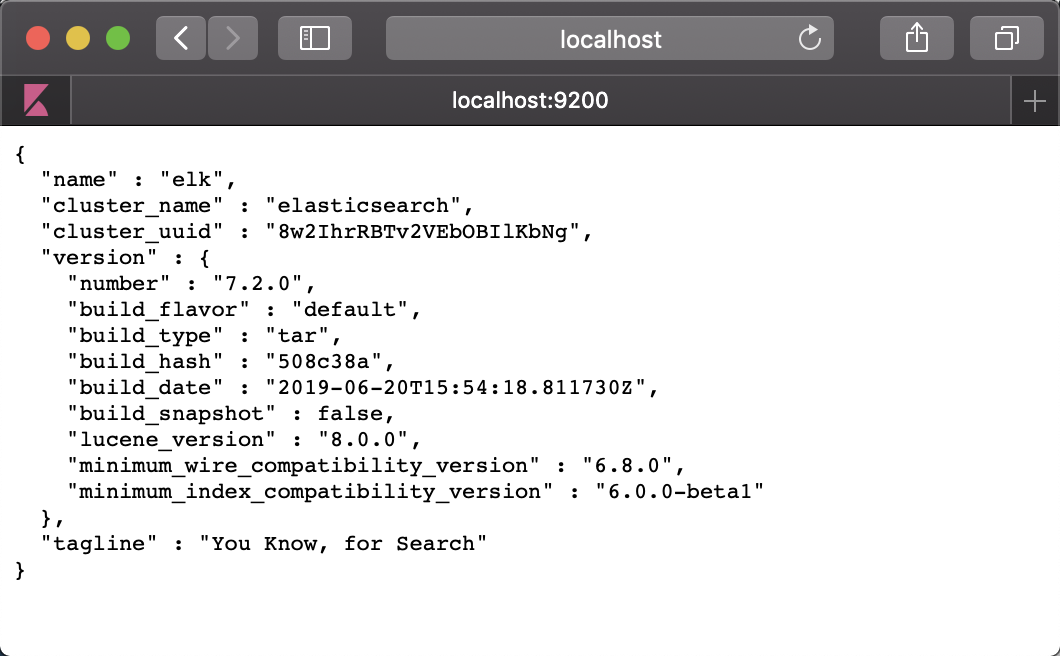
\includegraphics[scale=0.4 ]{images/elastic_return.png}
	\caption{Return Elasticsearch}
	\label{fig:return_elk}
\end{figure}

Anschliessend wird der Index, siehe Abbildung \ref{fig:elk_index}, und das Mapping, siehe Abbildung \ref{fig:elk_mapping} erstellt. Da es sich bei Elasticsearch um eine REST API handelt, kann entweder mit der  Kommandozeile oder mit einem API Tool wie \href{https://www.getpostman.com}{Postman} gearbeitet werden. F{\"u}r diese Arbeit wurde Postman verwendet, da die Arbeit mit dediziertem Tool komfortabler ist und das grosse Mapping in den JSON Requests / Antworten damit deutlich besser lesbar ist, als auf der Kommandozeile.

\begin{figure}[H]
	\centering
		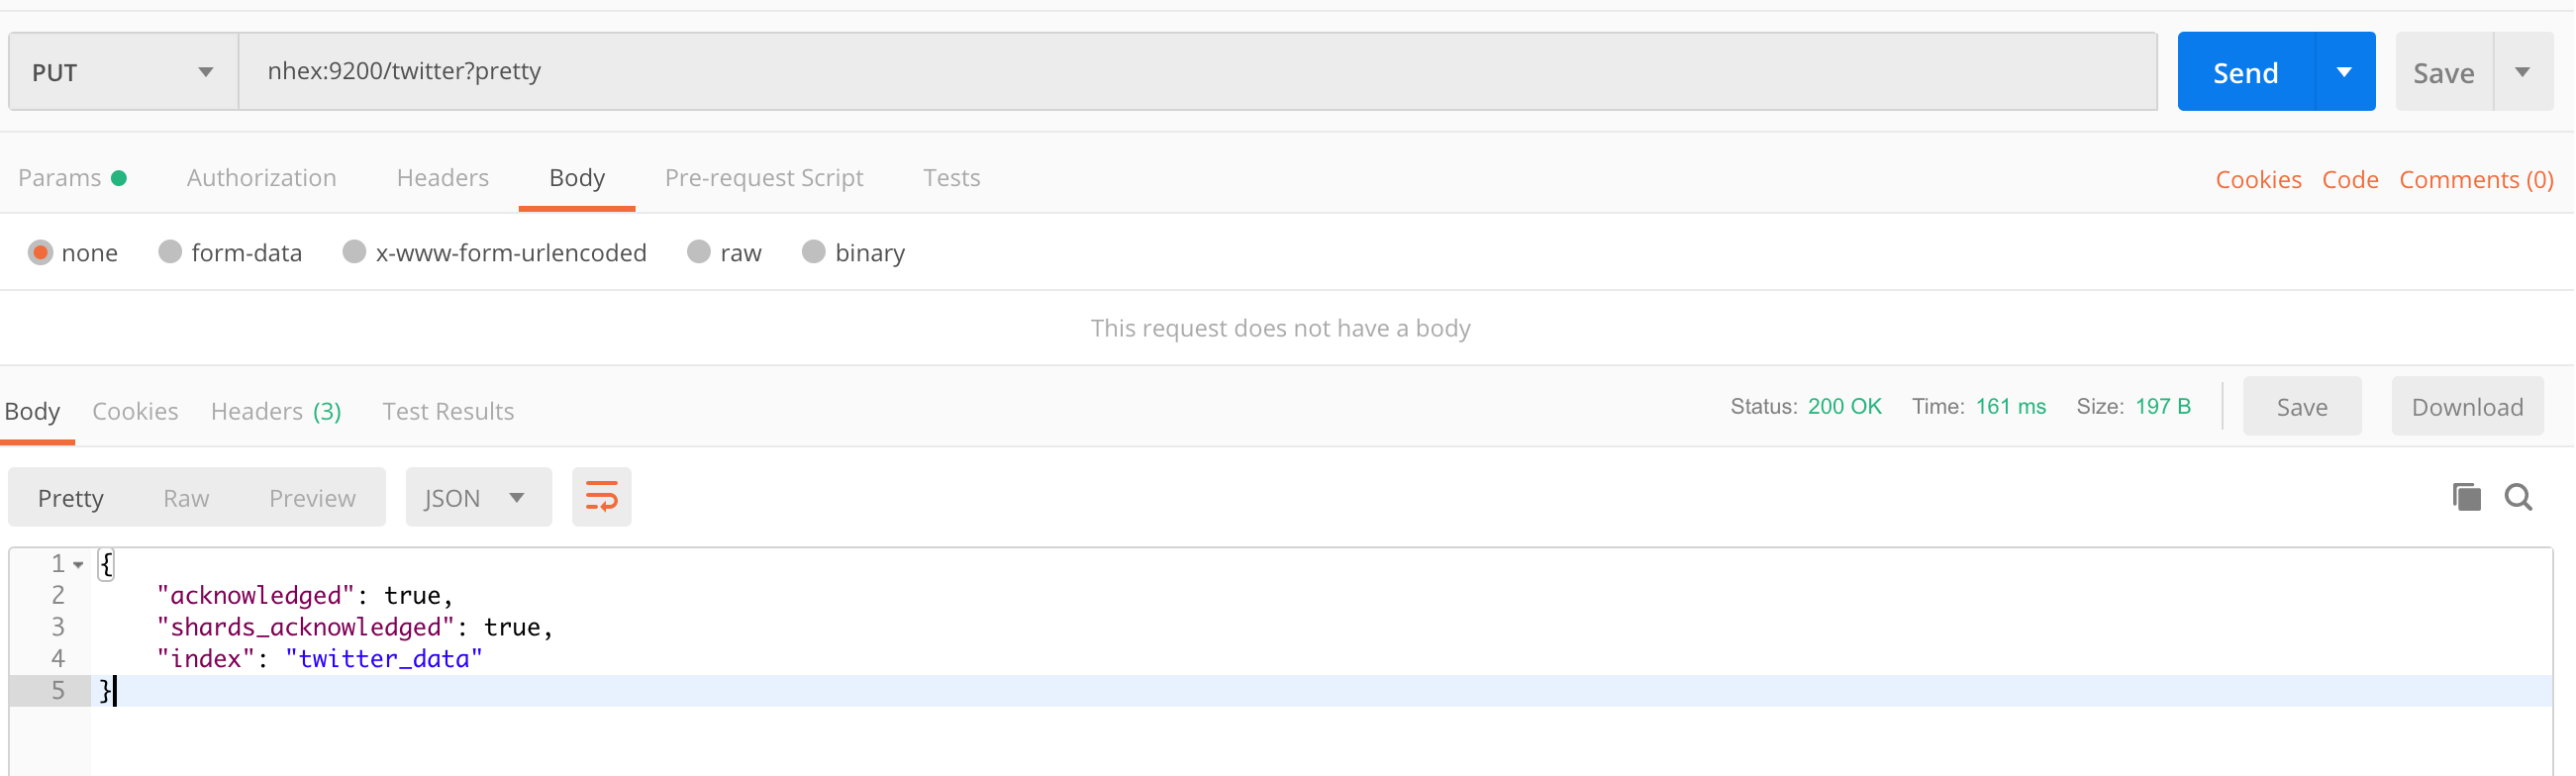
\includegraphics[scale=0.2]{images/elastic_create_index.png}
	\caption{Elastic: Erstellen eines Index}
	\label{fig:elk_index}
\end{figure}


\begin{figure}[H]
	\centering
		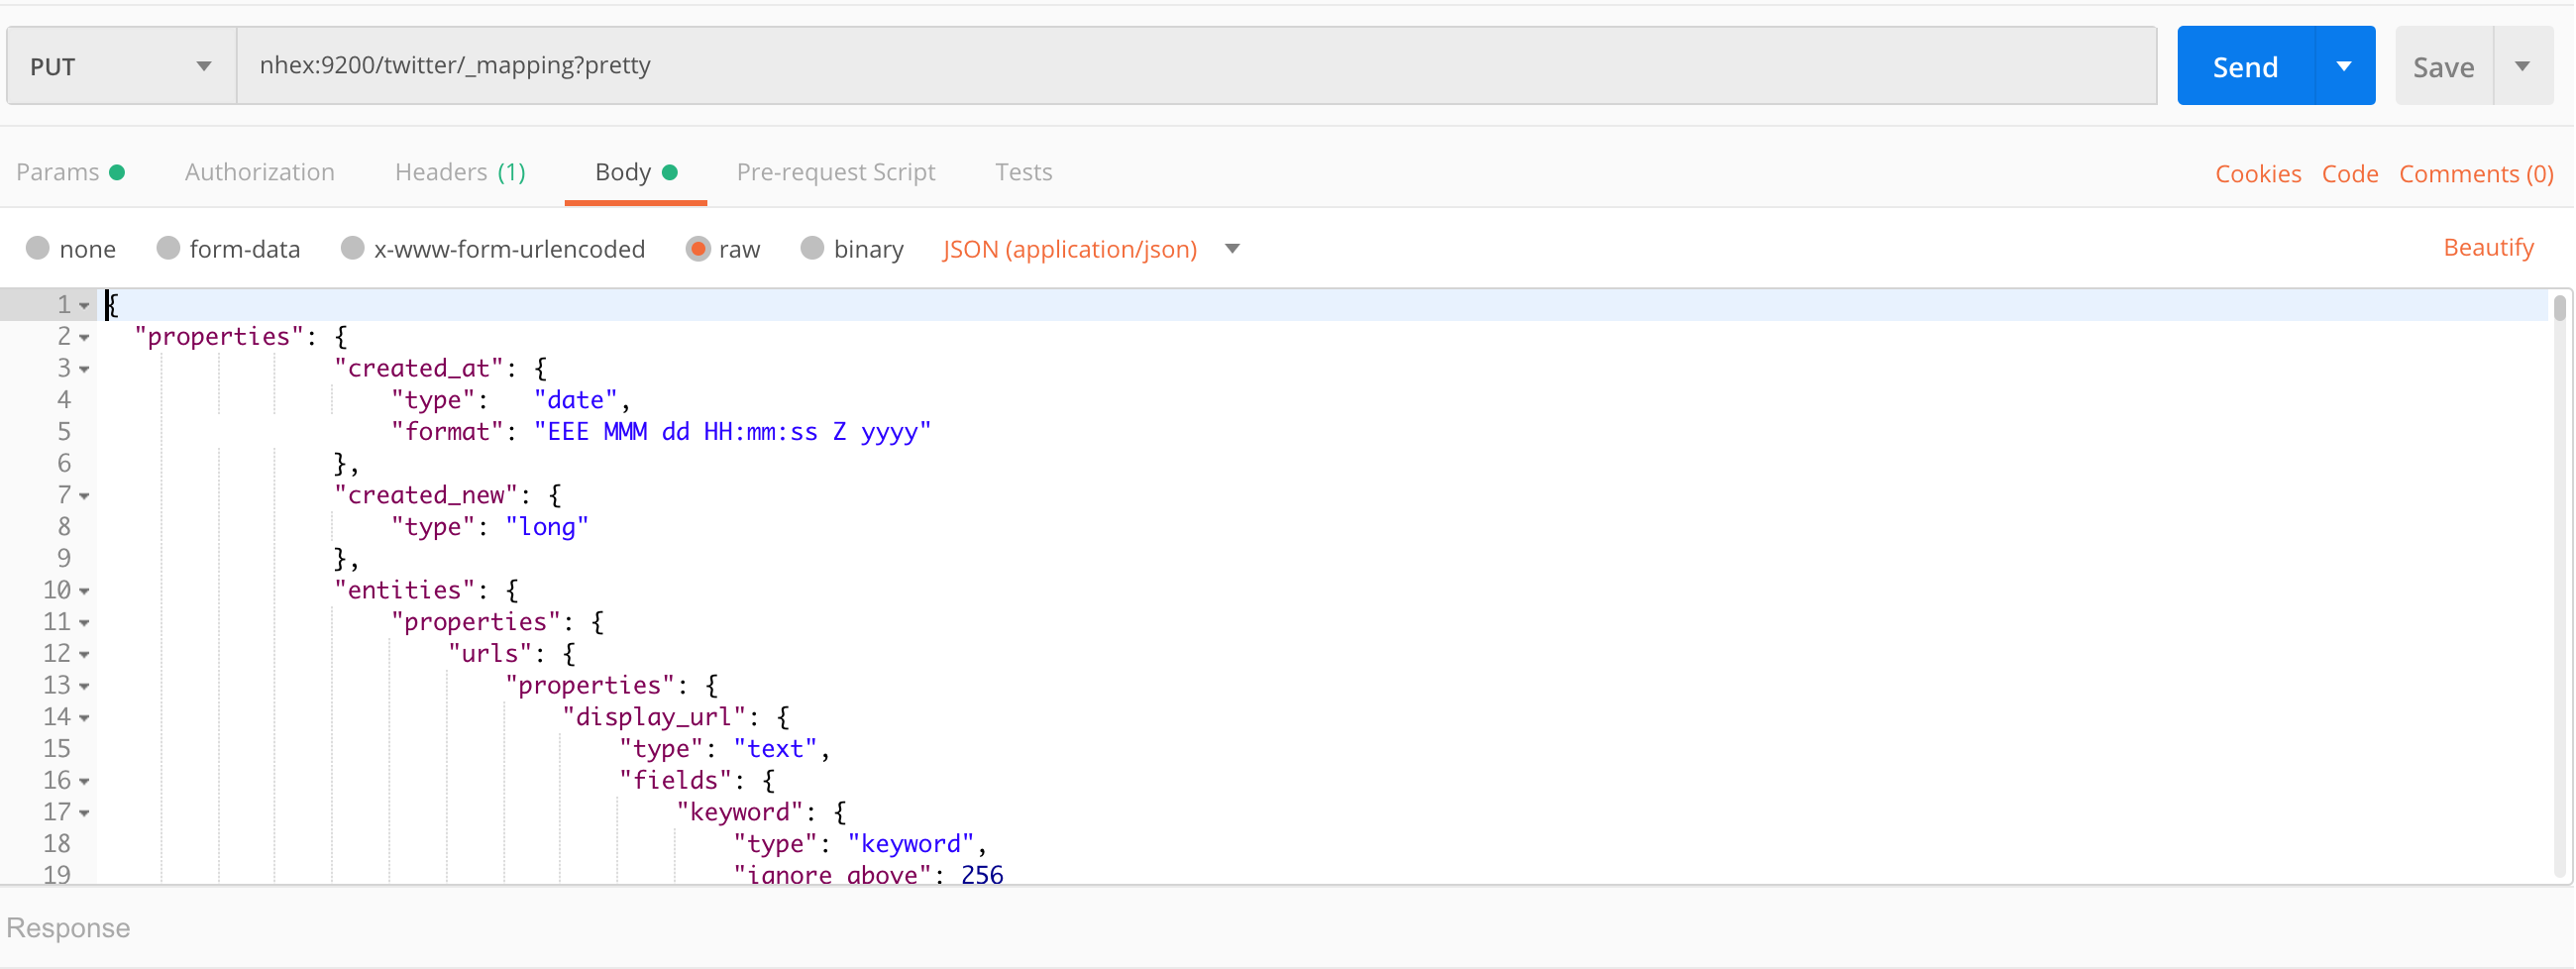
\includegraphics[scale=0.2]{images/elastic_create_mapping.png}
	\caption{Elastic: Erstellen eines Mappings}
	\label{fig:elk_mapping}
\end{figure}


\section{Pipeline Architektur}
\label{sec:pipeline_architecture}
Nachdem die Services konfiguriert und lauff{\"a}hig sind, werden die Pipelines aufgebaut. Anstatt eine einzelne Pipeline f{\"u}r alle Prozessschritte zu erstellen, werden mehrere Pipelines erstellt, was eine lose Kopplung der Prozesschritte beg{\"u}nstigt. Die Anzahl der zu erstellenden Pipelines ergibt sich aus der Anzahl der zu erledigenden Aufgaben:

\begin{itemize}
  \item Daten von Twitter streamen resp. einlesen
  \item Rohdaten von Twitter f{\"u}r die Masterarbeit in MongoDB speichern
  \item Rohdaten aufbereiten und Tweets klassifizieren
  \item Klassifizierte Tweets in Elasticsearch speichern
\end{itemize}

Mit dem Bau von mehreren Pipelines ist ein {\"A}ndern einzelner Schritte m{\"o}glich, ohne die komplette Verarbeitung zu stoppen resp. unterbrechen. Bei einer einzigen Pipeline, einem Monolithen, m{\"u}sste immer alles angehalten werden und es gingen Rohdaten von Twitter verloren. Durch den atomaren Aufbau und den Einsatz von Kafka, f{\"u}r die Kommunikation zwischen die Pipelines, k{\"o}nnen diese f{\"u}r {\"A}nderungen kurz gestoppt und wieder gestartet werden, ohne dass es sich auf die Daten resp. den Gesamtprozess auswirkt. 

Die kompletten Konfigurationen und die Pipelines sind in Github abgelegt und k{\"o}nnen in StreamSeats importiert werden.

\subsection{Daten von Twitter streamen}
\label{sec:collect_tweets}

\begin{figure}[H]
	\centering
		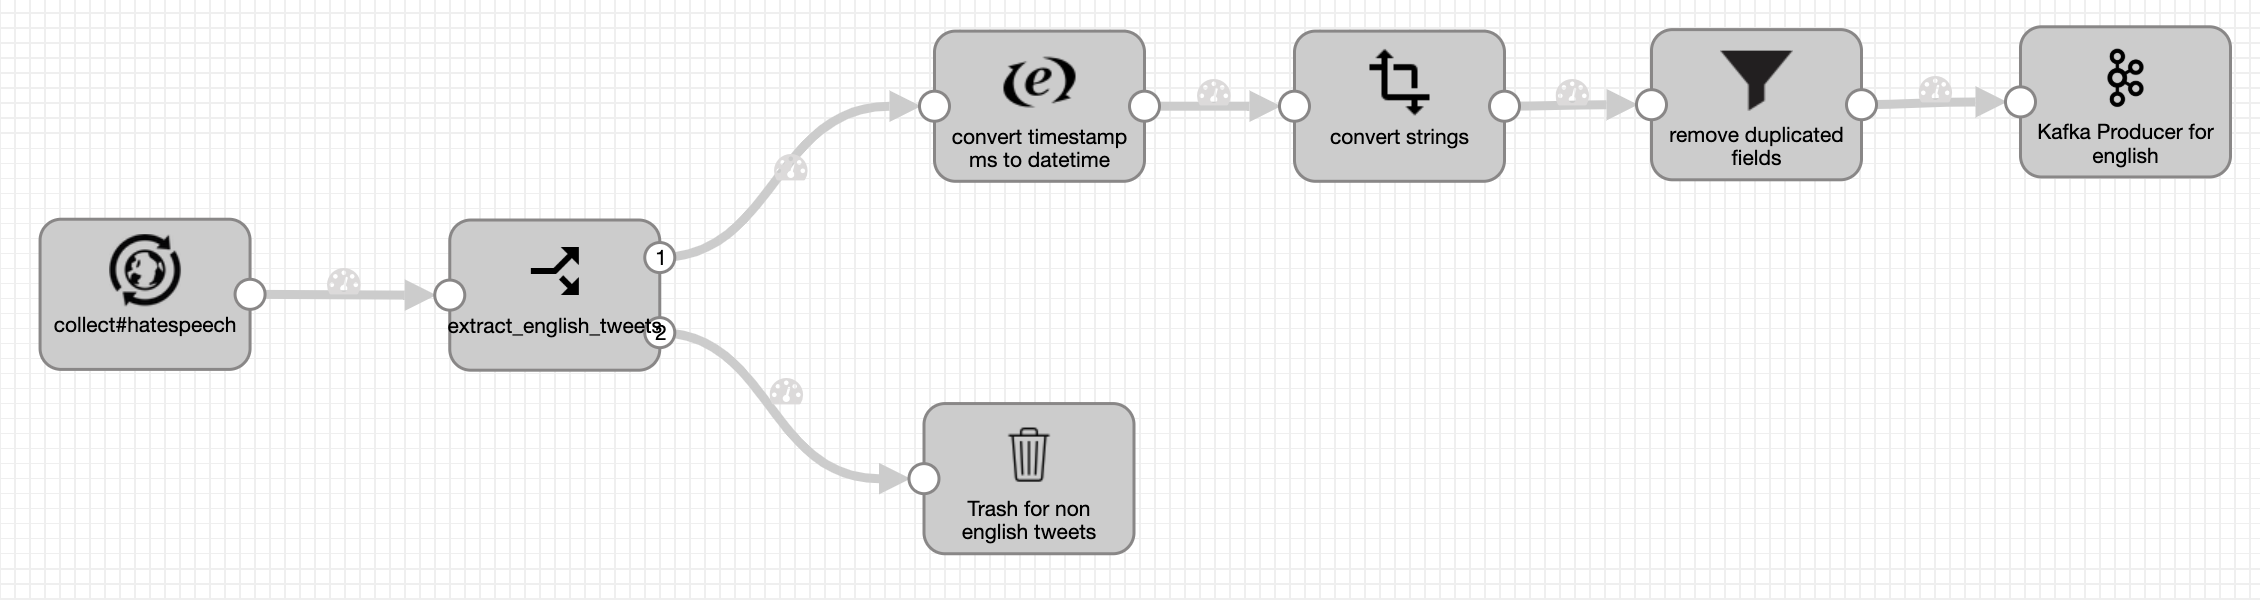
\includegraphics[scale=0.4 ]{images/pipeline_collect_tweets.png}
	\caption{Pipeline um Daten von Twitter zu bekommen}
	\label{fig:pipline_collect_tweets}
\end{figure}

Die Pipeline Daten von Twitter, Abbikdung \ref{fig:pipline_collect_tweets}, streamt Rohdaten von der Twitter API und  besteht aus folgenden Schritten:

\begin{itemize}
  \item http client um die Daten von der Twitter API zu beziehen. In dieser Semesterarbeit wird auf das Word Trump in Twitter Feeds gefiltert, um die gewaltige Menge von Twitter Feeds in eine verarbeitbare und dennoch gen{\"u}gend grosse Menge von Tweets einzuschr{\"a}nken. Die Twitter API l{\"a}sst nur ein streaming unter der Angabe von mindestens einem Parameter zu.
  \item Stream Seperator um die englischsprachigen Tweets zu filtern.
  \item Trash um die nicht englischsprechigen Tweets zu l{\"o}schen.
  \item Expression evaluator um den time stamp zu konvertieren
  \item Field converter um die Strings zu Ints zu konvertieren
  \item Field remover um nicht ben{\"o}tigte Felder zu l{\"o}schen
  \item Kafka Producer um die gesammelten englischen Rohdaten von Twitter in das Kafka Topic  \texttt{tweets\_eng} zu schreiben.
\end{itemize}
 

\subsection{Rohdaten in MongoDB}
\label{sec:tweets_to_mongo}

Die Pipeline Rohdaten in MongoDB, Abbildung \ref{fig:pipeline_tweets_to_mongo}, speichert die gesammelten Rohdaten von Twitter in eine MongoDB. 

\begin{figure}[H]
	\centering
		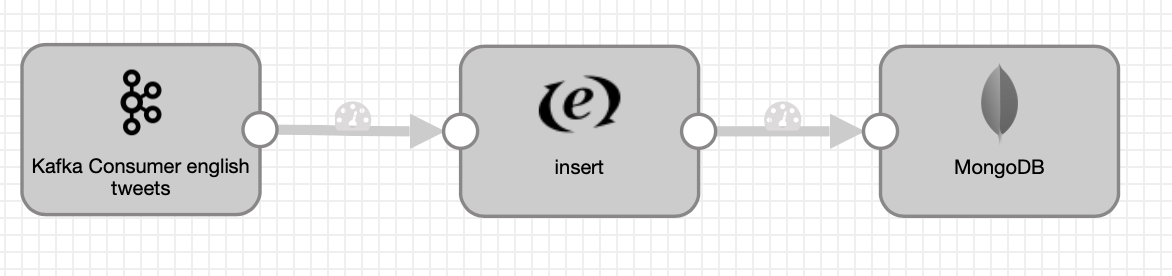
\includegraphics[scale=0.4 ]{images/tweets_to_mongo.png}
	\caption{Pipeline um Daten in MongoDB zu schreiben}
	\label{fig:pipeline_tweets_to_mongo}
\end{figure}

Diese Pipeline besteht aus drei Schritten:

\begin{itemize}
  \item Kafka Consumer um die Rohdaten von Twitter aus dem Kafka Topic \texttt{tweets\_eng} auszulesen
  \item Expression evaluator um die Operation f{\"u}r die MongoDB festzulegen. In diesem Fall das Schreiben der Daten, also ein insert.
  \item MongoDB um die Daten dort zu speichern.
\end{itemize}

\subsection{Rohdaten aufbereiten und Tweets klassifizieren}
\label{sec:predict_tweets}

Die Pipeline Rohdaten aufbereiten und Tweets klassifizieren, Abbildung \ref{fig:pipeline_predict_tweets}, bereinigt die Rohdaten, klassifiziert die Tweets mittels der detect-hate App und geocodiert die Herkunft der Benutzer mit Hilfe von HERE. 

\begin{figure}[H]
	\centering
		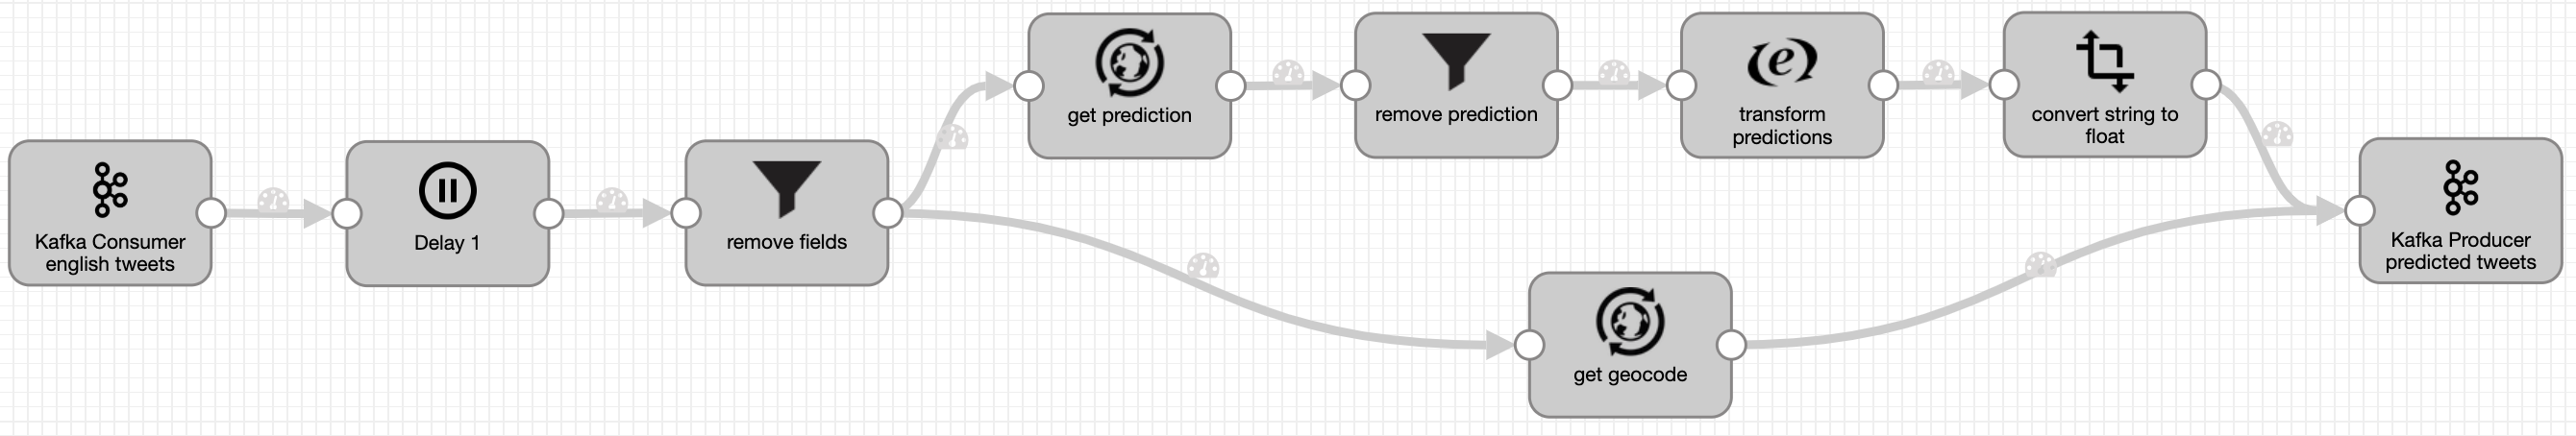
\includegraphics[scale=0.3]{images/pipeline_predict_tweets.png}
	\caption{Pipeline um die Tweets zu klassifizieren}
	\label{fig:pipeline_predict_tweets}
\end{figure}

Die folgenden Schritte werden in der Pipeline ausgef{\"u}hrt:

\begin{itemize}
  \item Kafka Consumer um die Rohdaten von Twitter aus dem Kafka Topic \texttt{tweets\_eng} auszulesen.
  \item Delay um die Anfragen, welche zu detect-hate.com geschickt werden zu verz{\"o}gern.
  \item Field remover um alle nicht ben{\"o}tigten Felder zu entfernen. 
  \item http client um den Tweet zur detect-hate App zu schicken und klassifizieren zu lassen.
  \item http client um die Location zu HERE zu schicken und geocodieren zu lassen.
  \item Field remover um nicht ben{\"o}tigte Felder, welche in der Antwort von der detect-hate App geschickt wurden zu entfernen.
  \item Expression evaluator um unerw{\"u}nschte Werte in den Wahrscheinlichkeiten zu entfernen.
  \item Field converter um die Wahrscheinlichkeiten von String in int zu konvertieren.
  \item Kafka Producer um die klassifizierten Daten in das Kafka Topic \texttt{predicted\_tweets} zu schreiben.
\end{itemize}

In einer weiteren Version der Pipeline wurde der Schritt Delay entfernt, da die detect-hate App von dem bisher verwendeten NAS ebenfalls auf den nHex portiert und gleichzeitig skaliert wurde. Dadurch steigt die Performance und die App kann die Klassifizierung bedeutend schneller vornehmen. 

\subsection{Klassifizierte Tweets in Elasticsearch}
\label{sec:tweets_to_elk}

Die Pipeline klassifizierte Tweets in Elasticsearch, Abbildung \ref{fig:pipeline_tweets_to_elk}, speichert die klassifizierten Tweets in elasticsearch.

\begin{figure}[H]
	\centering
		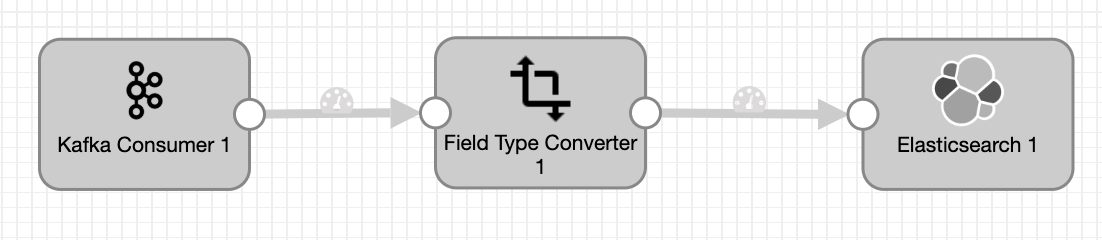
\includegraphics[scale=0.4 ]{images/pipeline_tweets_to_elk.png}
	\caption{Pipeline um die Tweets zu klassifizieren}
	\label{fig:pipeline_tweets_to_elk}
\end{figure}

Die folgenden Schritte werden in der Pipeline ausgef{\"u}hrt:

\begin{itemize}
  \item Kafka Consumer um die Daten aus dem Kafka Topic \texttt{predicted\_tweets} auszulesen.
  \item Expression evaluator um ein timestamp passend f{\"u}r elasticsearch zu konvertieren.
  \item Elasticsearch um die Daten zu speichern. 
\end{itemize}

\section{Dashboard}
\label{sec:dashboard}
Das Dashboard ist in mehrere thematisch zusammenh{\"a}ngende Anschnitte aufgeteilt und besteht Gesamthaft aus 24 einzelnen Visualisierungen. Nachfolgend werden einige interessante  Visualisierungen beschrieben. In Abbildung \ref{fig:kibana_1} sind allgemeine Informationen zu den Tweets zusehen:

\begin{itemize}
  \item Gesamte Anzahl Tweets im aktuell selektierten Zeitraum
  \item Unique Anzahl Hashtags dieser Tweets
  \item Unique Anzahl erw{\"a}hnter Benutzer in den Tweets
  \item Wordcloud mit den 50 h{\"a}ufigsten Hashtags
  \item Wordcloud mit den am 50 h{\"a}ufigst genannten Benutzern
  \item Diagramm mit den verwendeten absoluten Hashtags im Zeitverlauf
\end{itemize}


\begin{figure}[H]
	\centering
		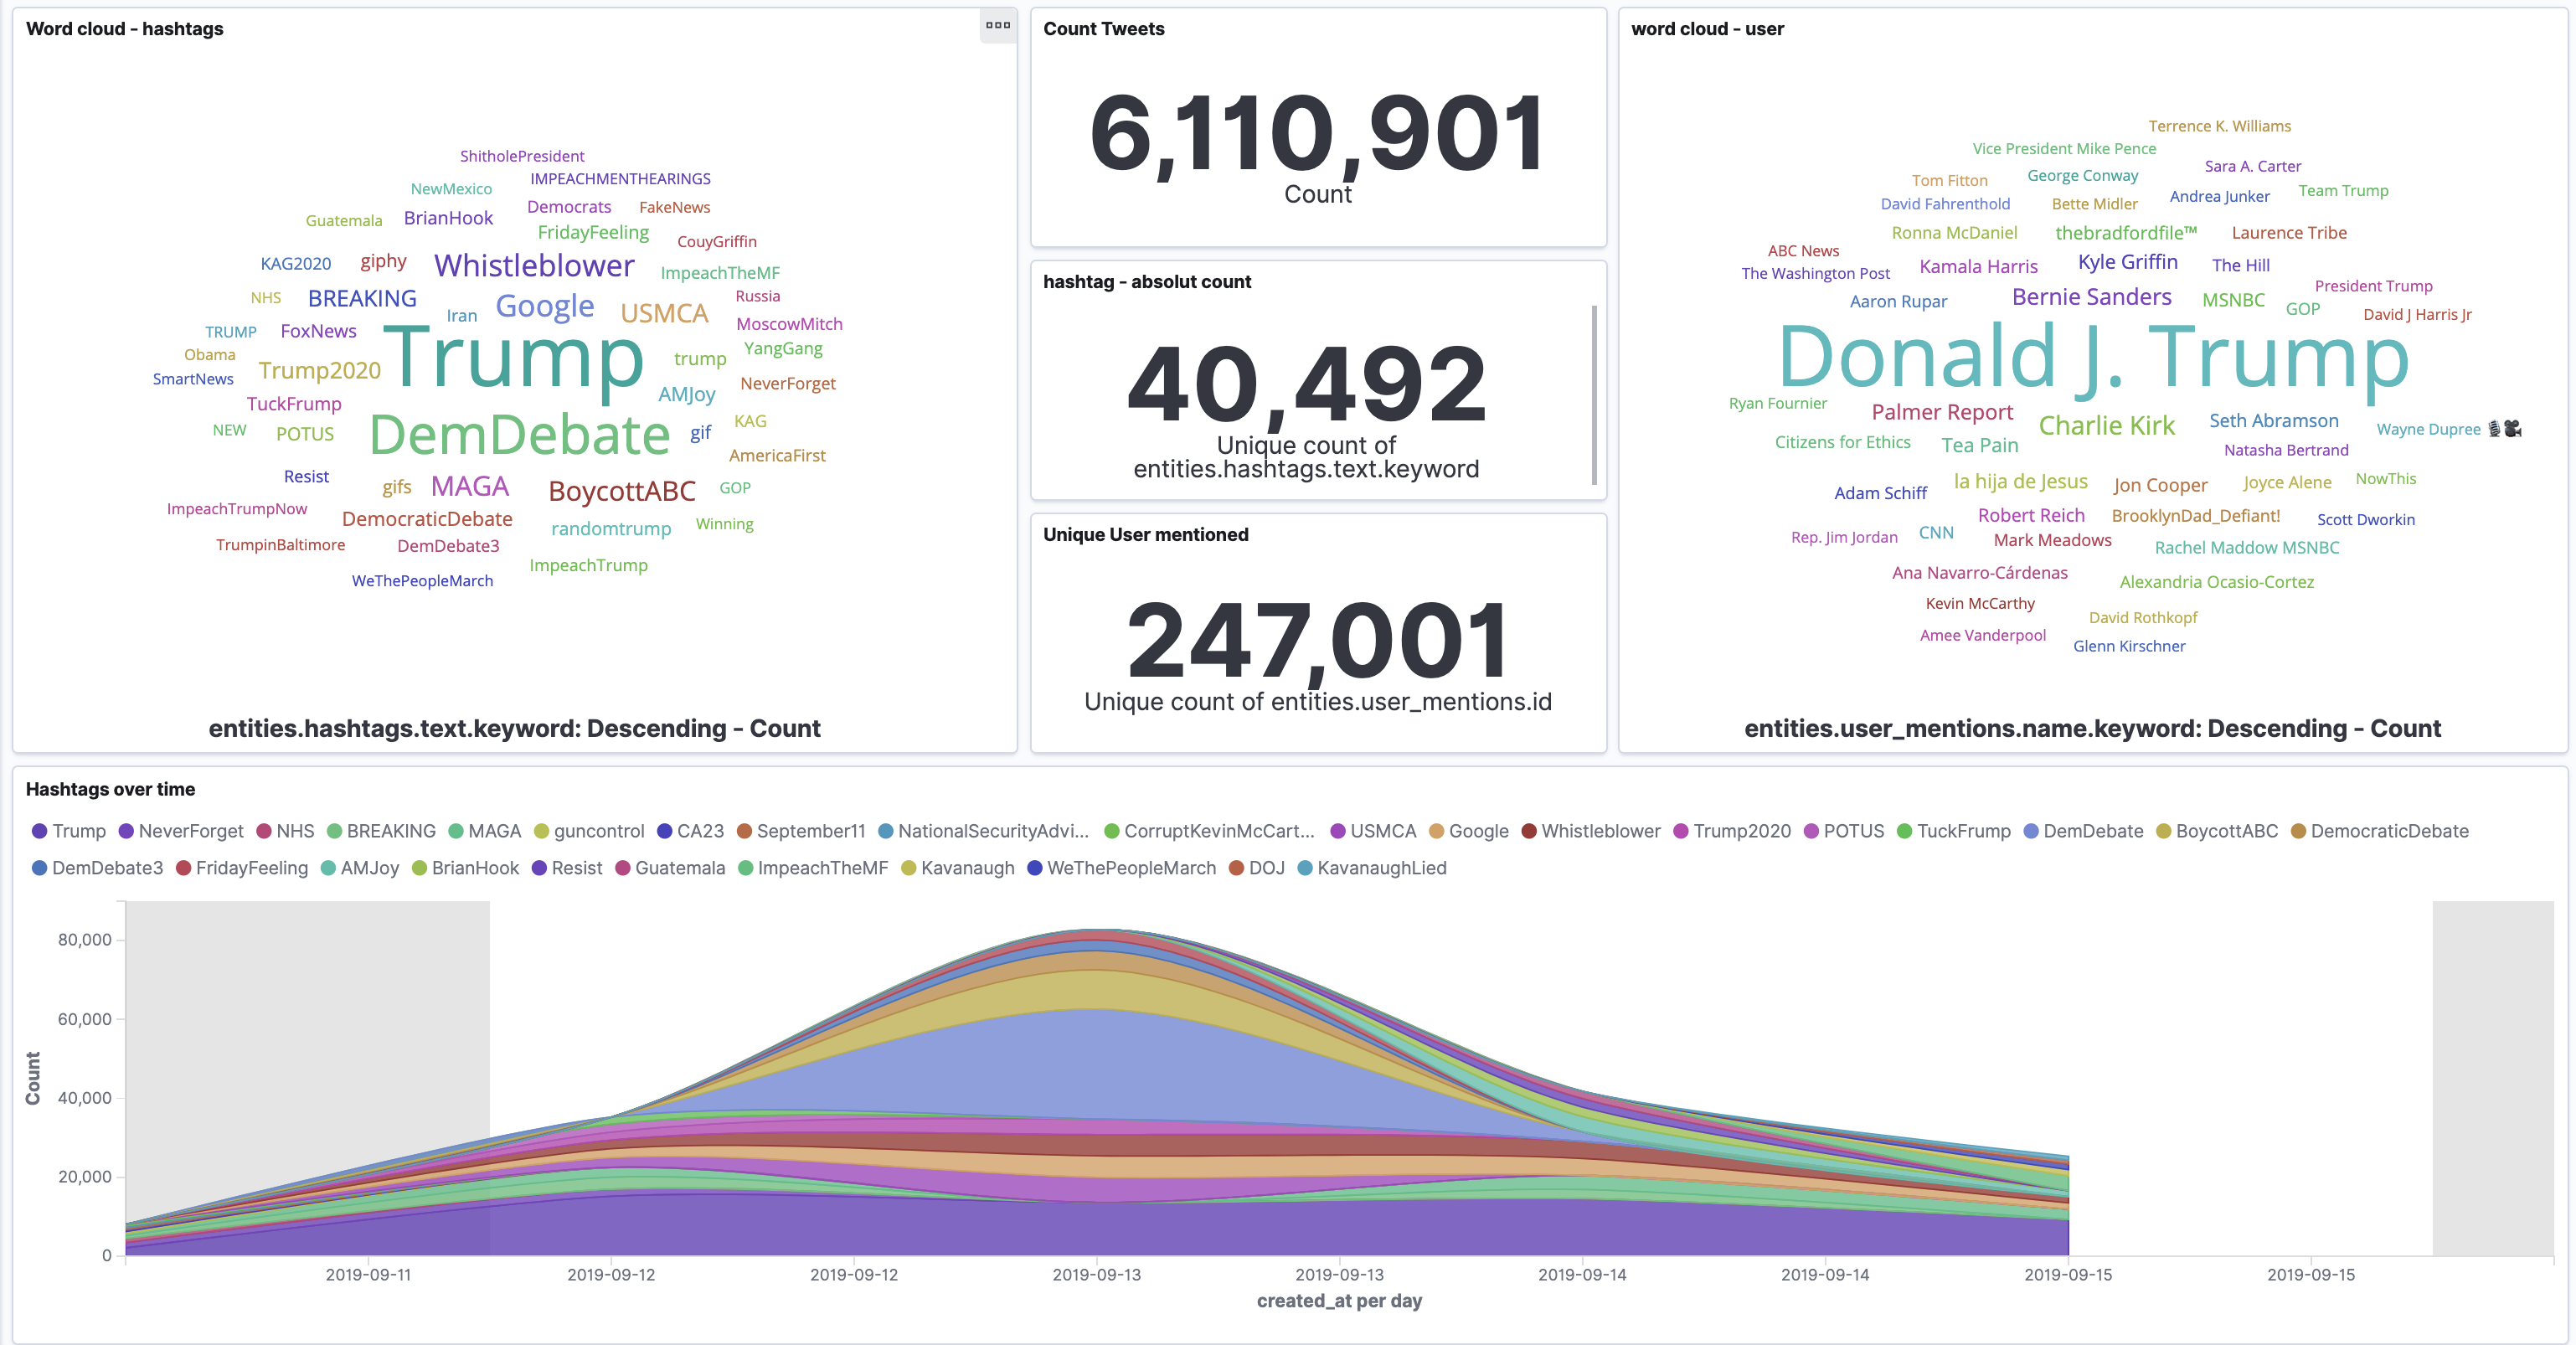
\includegraphics[scale=0.3]{images/kibana_dash_1.png}
	\caption{Auszug Kibana Dashboard allgemeine {\"U}bersicht}
	\label{fig:kibana_1}
\end{figure}

In Abbildung \ref{fig:kibana_2} ist die Anzahl der klassifizierten Tweets pro Modell ersichtlich. Dabei f{\"a}llt aus, das Linear SVM, logistic Regression und LSTM zwischen 15 und 20 Pronzent aller Tweets als abusive (also als Hasskommentare enthaltend) klassifizieren. Der Multinominal Naive Bayes classifier hingegen klassifiziert sogar ca. 30 Prozent als abusive. F{\"u}r weitere Analysen hierzu fehlte jedoch die Zeit, denn daf{\"u}r m{\"u}ssten die Tweets manuell gepr{\"u}ft und die Klassifikationen validiert werden. Ebenfalls dargestellt in dieser Abbildung sind die Aufteilung der verwendeten Clients (Ger{\"a}t, von welchem ein Tweet versendet worden ist, also iPhone, Browser, etc.) und ein Histogramm der meist 10 h{\"a}ufigst genannten Twitter User sowie die abosolute Verteilung der 10 h{\"a}ufigst genannten Hashtags.

\begin{figure}[H]
	\centering
		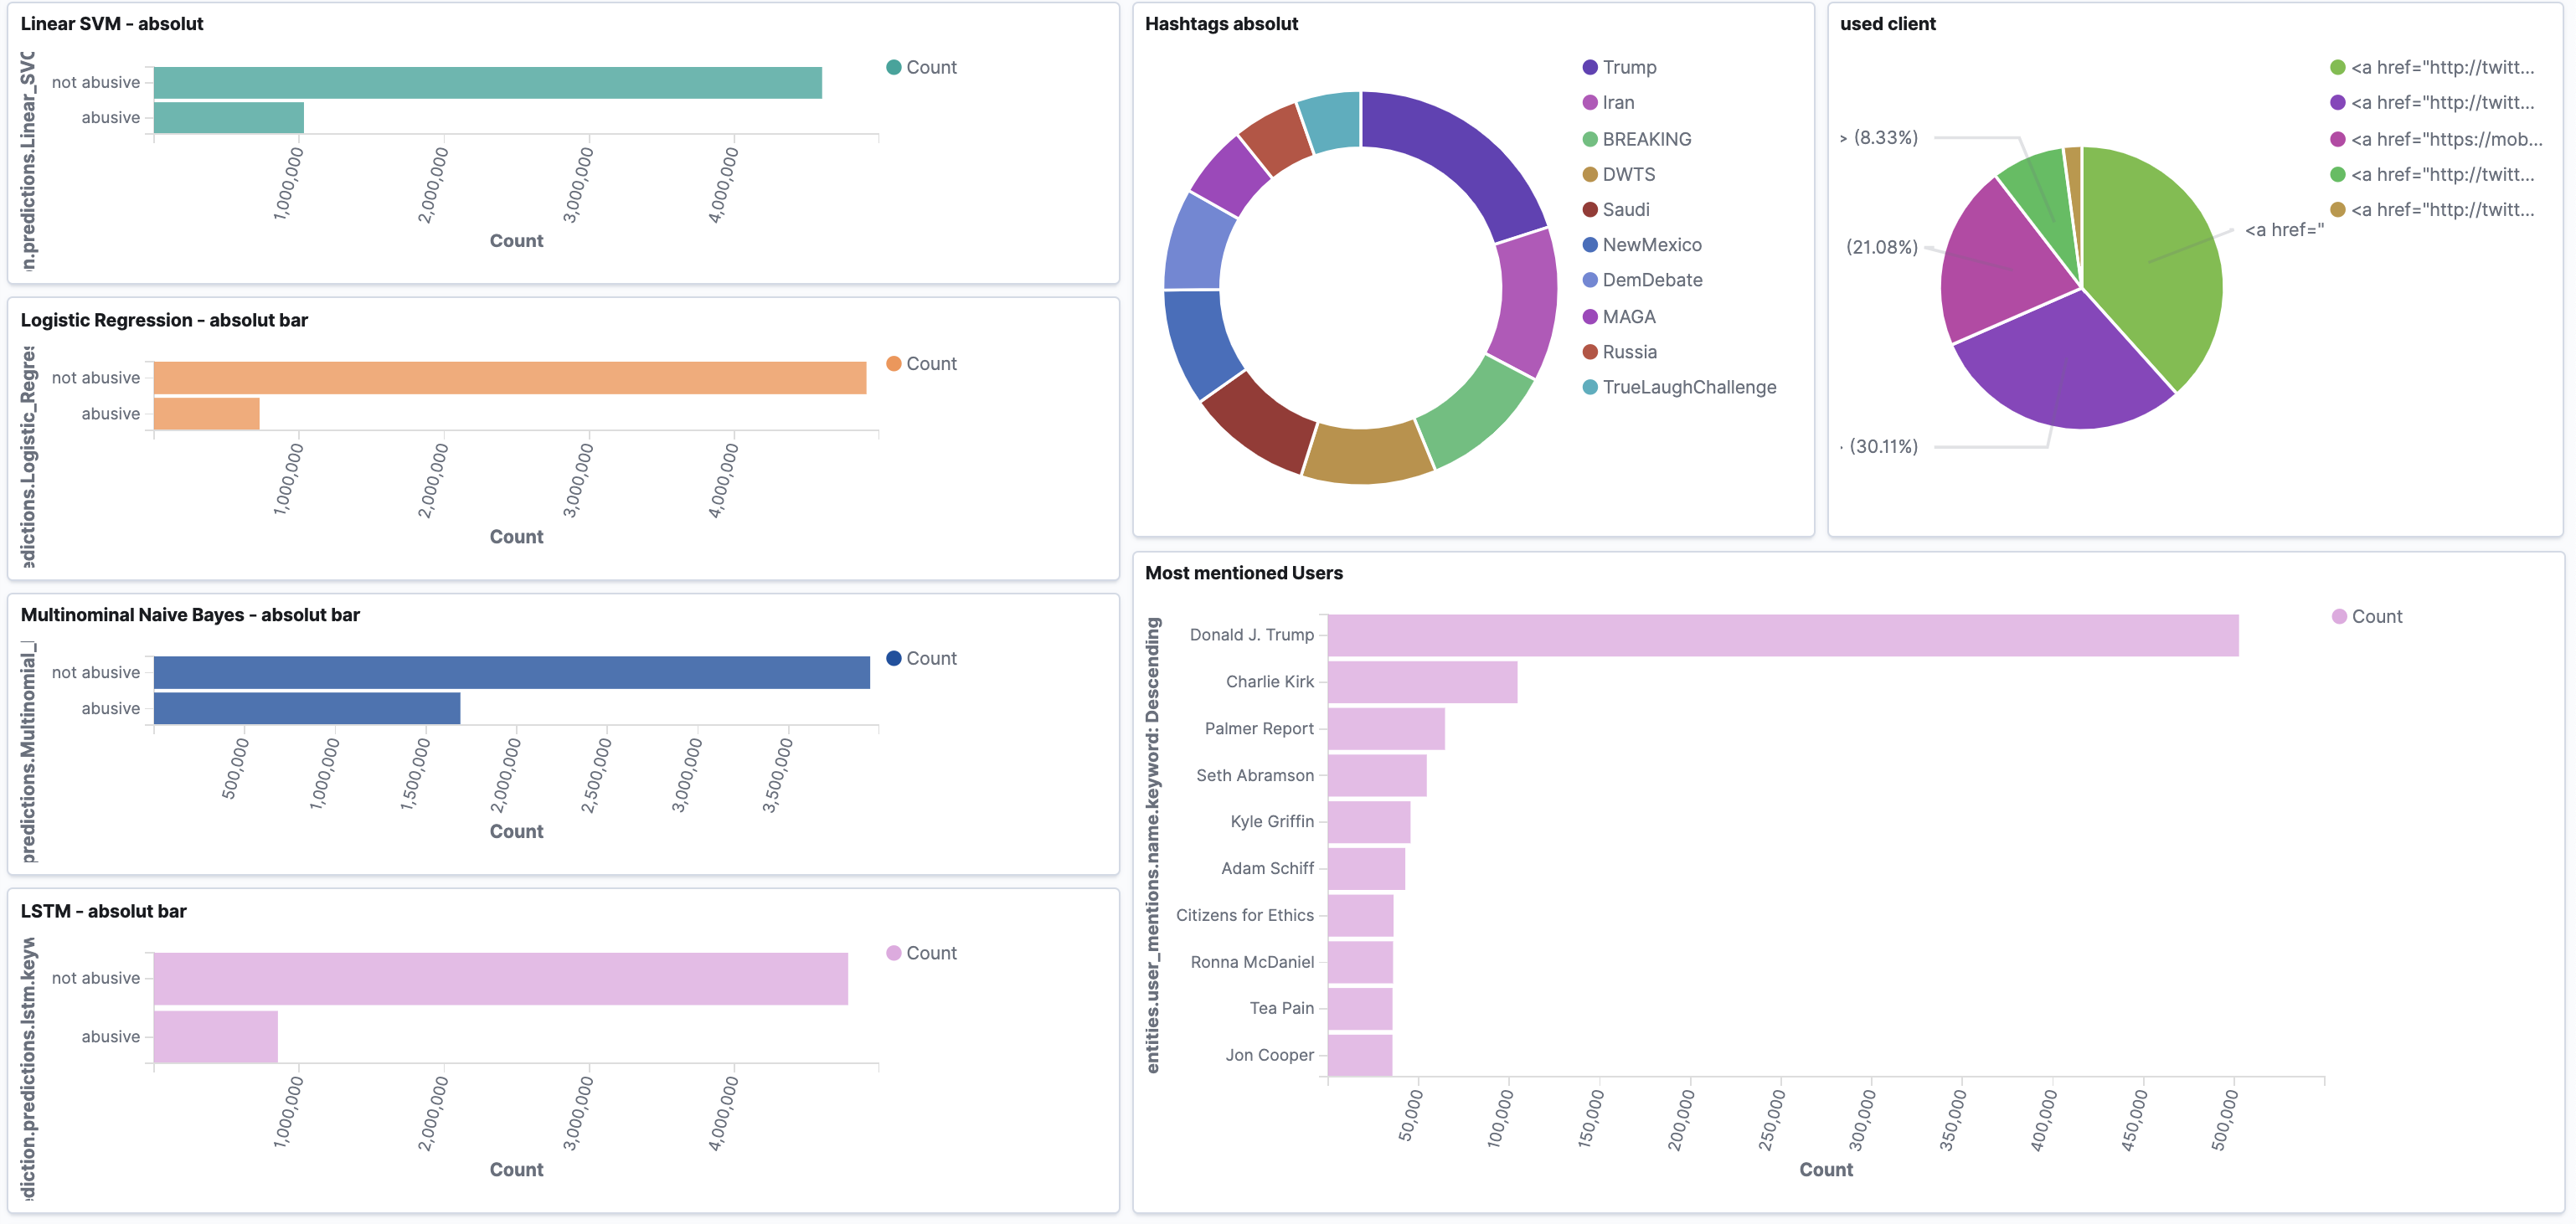
\includegraphics[scale=0.3]{images/kibana_dash_3.png}
	\caption{Auszug Kibana Dashboard Klassifikation}
	\label{fig:kibana_2}
\end{figure}

In Abbildung \ref{fig:kibana_3} ist als erstes die Gesamtanzahl der get{\"a}tigten Tweets pro Stunde abgebildet. In den vier unteren Balkendiagrammen sind die get{\"a}tigten Tweets pro Stunde nach ihrer Klassifizierung abgebildet. Ein Diagramm pro Modell. Auf allen Diagrammen ist der Tagesverlauf in den USA, wo am meisten Tweets verschickt werden, zu erkennen. Nachts in den USA sinkt die Anzahl der Tweets deutlich; zwar werden auch im Rest der Welt englische Tweets mit Trump als Textinhalt verschickt, einfach deutlich weniger. Interessanterweise scheint tags{\"u}ber mehr abusive klassifiziert zu werden. Es gilt noch zu verifizieren ob das auch nach einer Normalisierung noch zutrifft, ob dieses Verhalten nur absolut betrachtet auftritt, oder ob die Tweets in den Nachtstunden der USA von anderen Gegenden der Welt aus geschickt werden und dort eine weniger aggressive Ausdrucksweise verwendet wird. 

\begin{figure}[H]
	\centering
		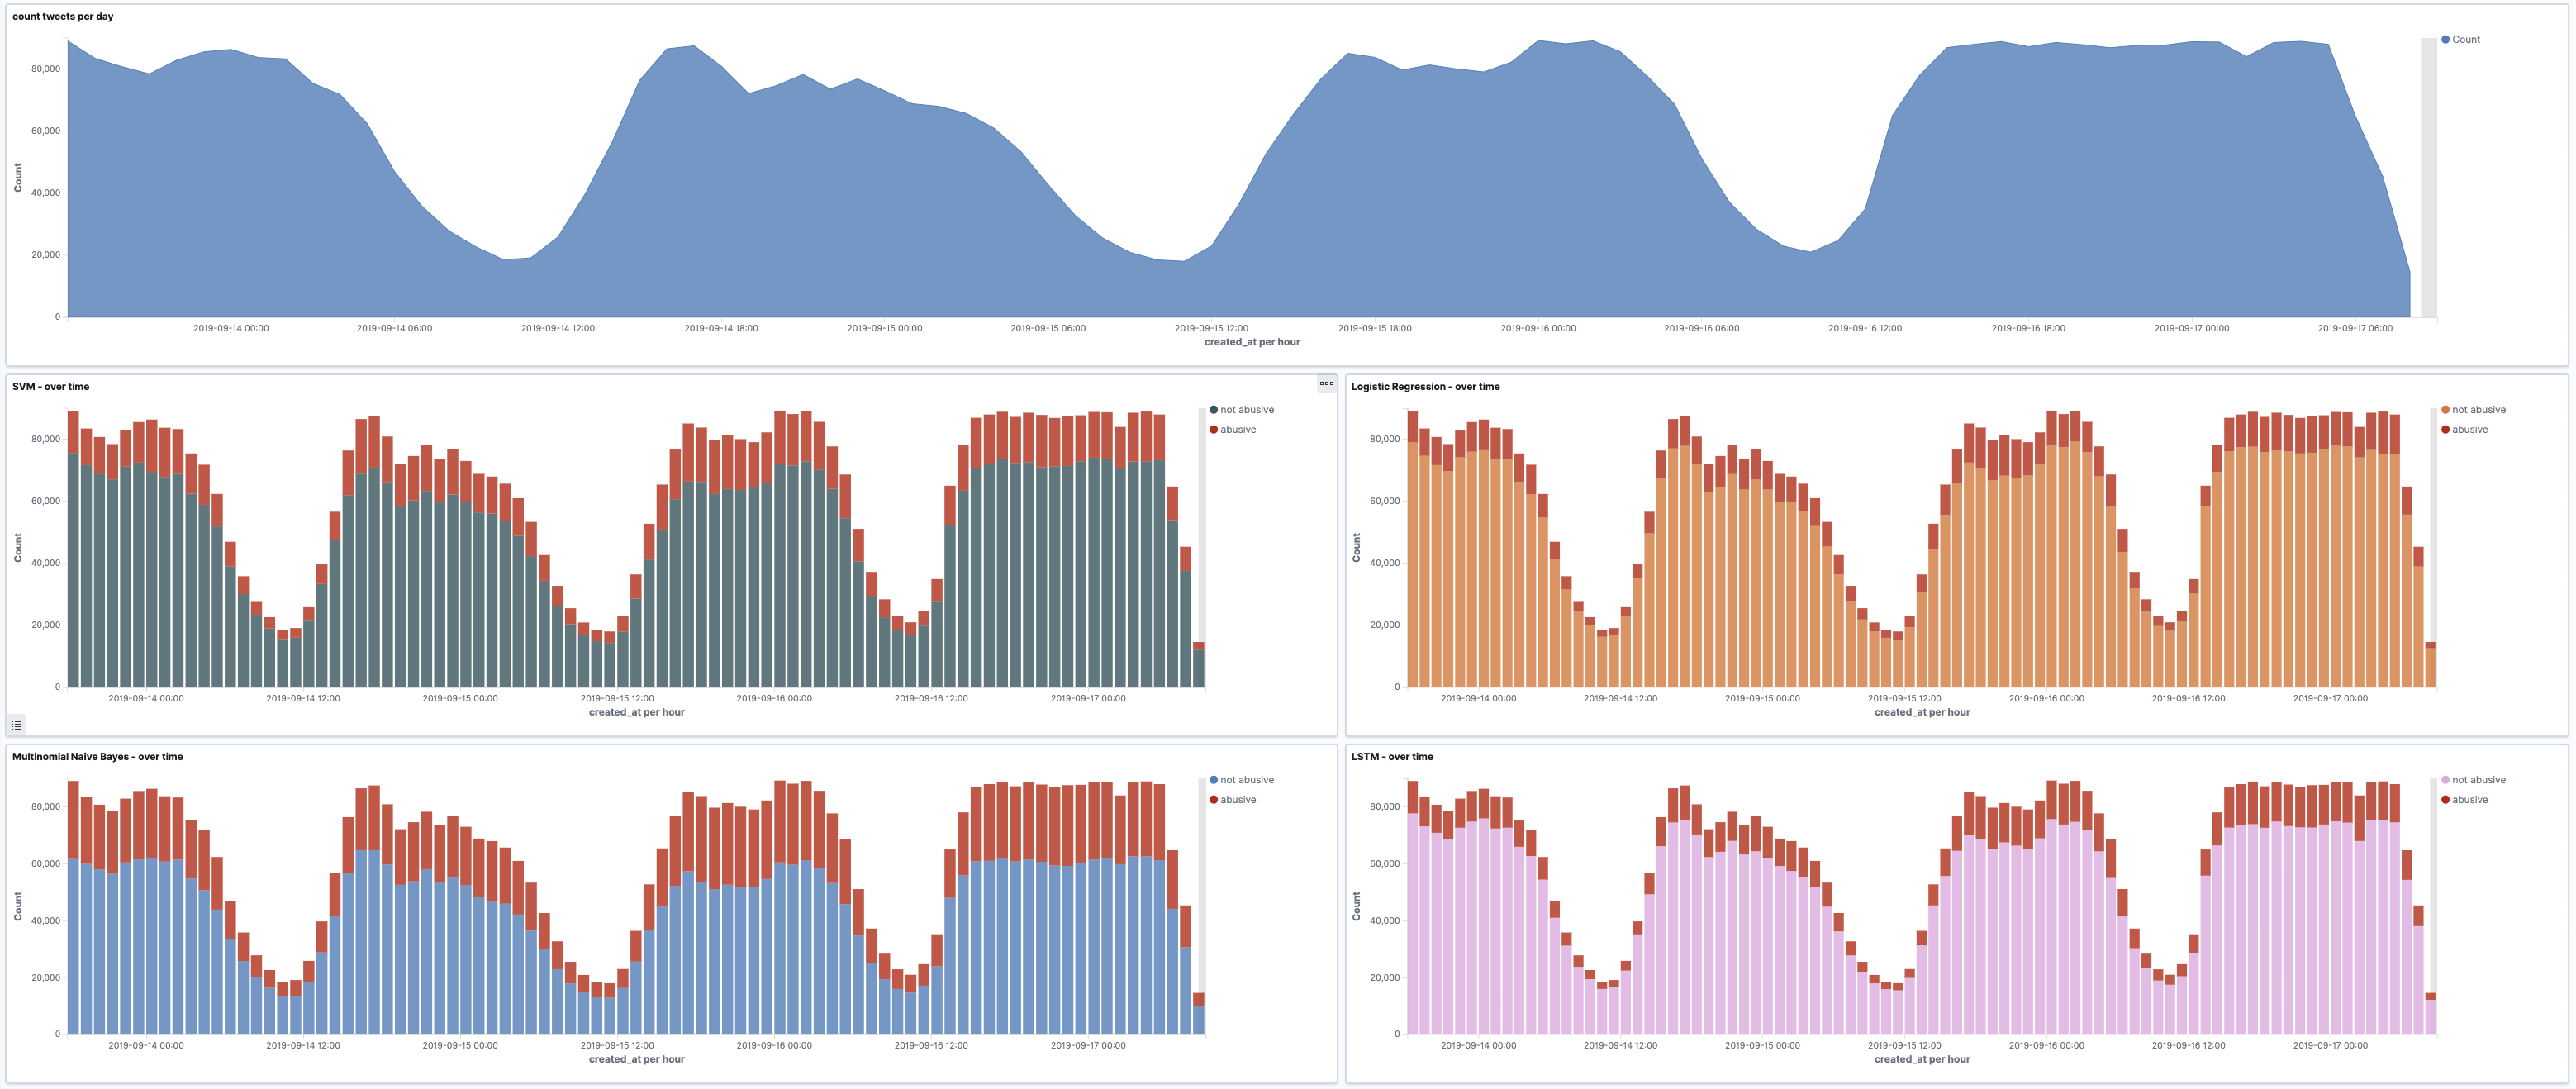
\includegraphics[scale=0.3]{images/kibana_dash_ab_noab1.png}
	\caption{Auszug Kibana Dashboard Klassifikation im Tagesverlauf}
	\label{fig:kibana_3}
\end{figure}

\section{Anpassungen an der API}
\label{sec:anpassung_api}
Damit mit der im CAS PML entwickelten detect-hate App Tweets via Pipeline automatisiert klassifiziert werden k{\"o}nnen, musste ein zus{\"a}tzlicher REST Endpunkt erstellt werden. Dieser Endpunkt ist auf \linebreak \texttt{http://www.detect-hate.com:12345/predict\_sentence} erreichbar. Zu Testzwecken kann ein einzelner Tweet (resp. beliebiger englischer Text) mit dem Parameter \texttt{input\_text} an diesen Endpoint {\"u}bermittelt werden. Abbildung \ref{fig:ppostman_post} zeigt einen exemplarischen Aufruf w{\"a}hrend der Endpoint Entwicklung der App in Postman (lokal getestet in der Abbildung). 

\begin{figure}[H]
	\centering
		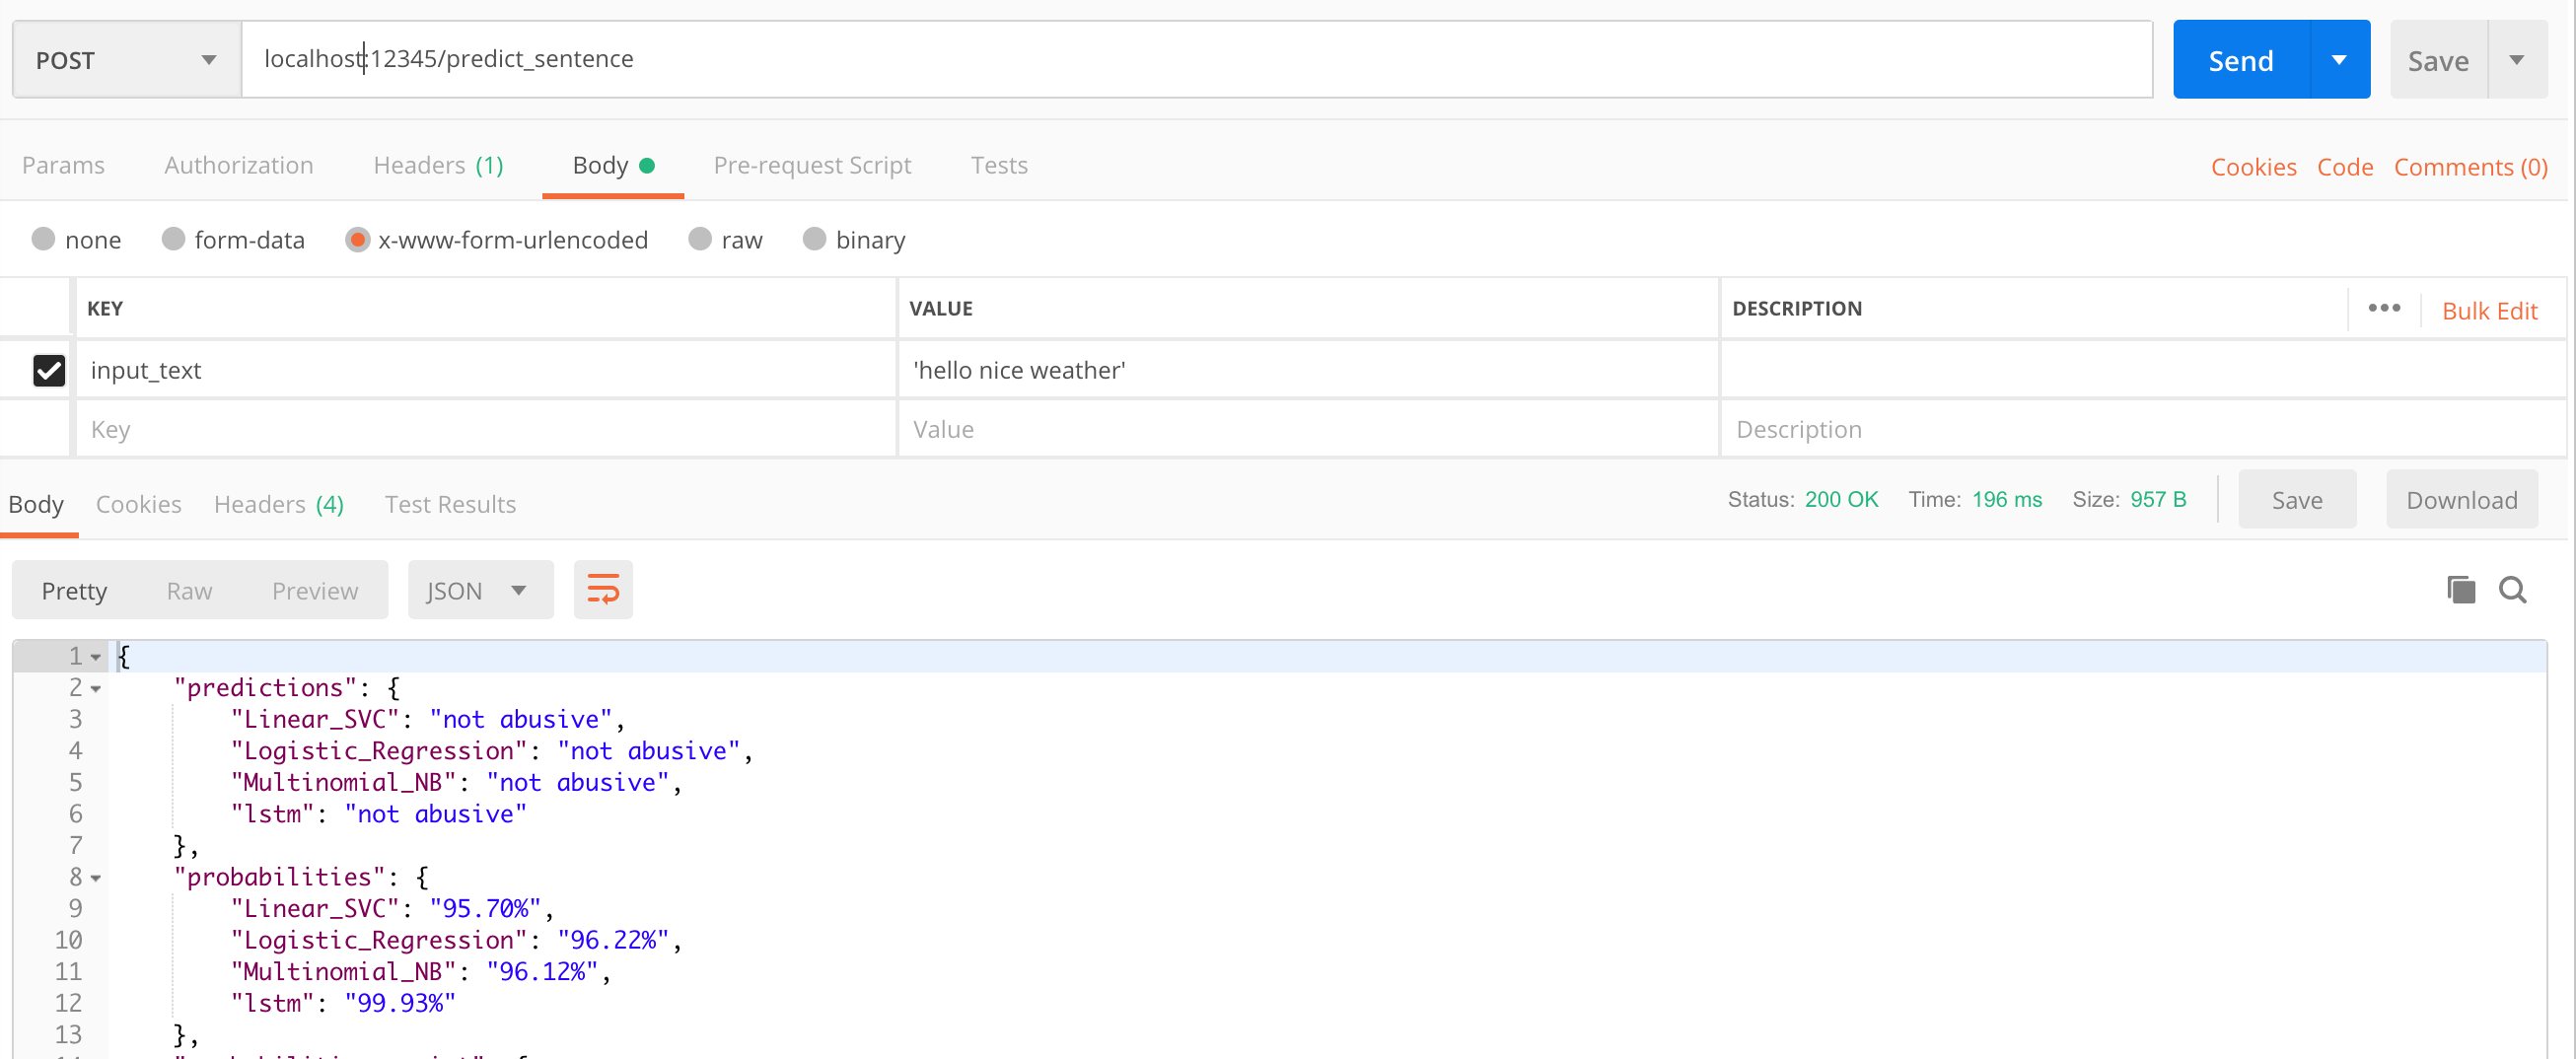
\includegraphics[scale=0.3]{images/postman_app.png}
	\caption{POST Request detect-hate App}
	\label{fig:ppostman_post}
\end{figure}

Nachdem die Pipelines erstellt und die API angepasst waren, hat sich bei den Tests mit gr{\"o}sseren Datenmengen herausgestellt, dass die detect-hate Klassifikation nicht robust und performant genug lief. Es gab immer wieder sporadisch Probleme mit der Erreichbarkeit der einzelnen Services. Nachdem jeweils circa 28.000 Datens{\"a}tze von Twitter gesammelt wurden, jedoch erst ca. 3.000 von diesen Daten klassifiziert waren, starteten sich die Services neu. Zwar liefen die Pipelines nach dem Neustart automatisch weiter, jedoch war der Zustand weder stabil, noch haltbar. 

Eine Analyse hat ergeben, dass die Last auf dem NAS zu hoch war und die detect-hate App nicht mit dem Klassifizieren hinterher kam. Um dieses Probelm zu beheben wurde zuerst die Pipeline angepasst; zum einen wurde ein Delay eingef{\"u}gt, zum anderen wurden Batches f{\"u}r die Verarbeitung definiert. Nachdem diese Anpassung nur zu einer geringf{\"u}gigen Verbesserung f{\"u}hrte wurde die App vom NAS auf den nHex portiert und skaliert. Da der nHex einerseits {\"u}ber die bessere Hardware verf{\"u}gt und andererseits die App Dank Kubernetes auf mehreren Nodes skaliert werden konnte, verbesserte sich die Performance der Klassifizierung um ein Vielfaches und erlaubt nun die Klassifizierung vonTweets in beinahe Echtzeit.

\section{Installation auf dem nHex}
\label{sec:nHex}

Die Spezifikation des BigBoards Cluster 'nHex i3' ist in Tabelle \ref{tab:spez_hnex} beschrieben.

\begin{table}[H]
	\centering
		\begin{tabular}{lll} 
			number of nodes & 6 \\ \midrule
			system platform  & Intel NUC \\ \midrule
			processor architecture & X86 64 \\ \midrule
			CPU & Intel Core i3 \\ \midrule
			number of cores & 12 cores \\ \midrule
			simultanious threads & 24 threads \\ \midrule
			DD3 RAM memory & 96 GB \\ \midrule
			2.5 HDD @ 7.2K RPM storage & 6 TB \\ \midrule
			integrated switch & 1 GB \\ \midrule
			external ethernet ports & 2 \\ \bottomrule
		\end{tabular}
	\caption{Spezifikation des nHex i3 Clusters}
	\label{tab:spez_hnex}
\end{table}
 
Um die Streaming und Analyse Umgebung auf den nHex zu portieren waren folgende Schritte n{\"o}tig:

\textbf{Installation eines neuen Betriebssystems}

Installation  von Ubuntu-Server 18.04 als Core OS auf allen Nodes. Daf{\"u}r wurde die Core Installation auf einen USB Stick geladen. Anschliessend jeden einzelnen Node in das BIOS starten und dort den Startup per USB Stick aktivieren. Nachdem dieses Anpassung in der Konfiguration gemacht wurde, konnte mit dem eigentlichen installieren des neuen Betriebssystem begonnen werden. Hierf{\"u}r wurde jeder Node vom USB Stick gestartet und die Installation durchgef{\"u}hrt. Anschliessend wurde jedem Node ein Name vergeben, ein Benutzer eingerichtet und SSH aktiviert.

Damit die Nodes immer die gleiche IP haben wurde auf der Fritz!Box (ein Router der Firma AVM) in den DHCP Settings die entsprechende Konfiguration aktiviert.

\textbf{Installation von Kubernetes}

F{\"u}r diese Arbeit wird \href{https://k3s.io}{K3s} verwendet, eine leichtgewichtige Version von Kubernetes. K3s eignet sich f{\"u}r kleinere Big Data Cluster, wie den nHex. Die Installation ben{\"o}tigt deutlich weniger Speicherplatz sowie Ressourcen und das Konfigurieren des Clusters erfolgt einfacher und komfortabler, als mit klassischem Kubernetes (k8s).

Zuerst wird f{\"u}r die Installation ein Node als Master bestimmt. Auf diesem wird die Installation als erstes durchgef{\"u}hrt. Anschliessend wird die Installation von K3s auf jedem weiteren der 5 verbleibenden Nodes des nHex als Agent durchgef{\"u}hrt und daf{\"u}r die entsprechenden Umgebungsvariablen gesetzt. 

Um mehr Komfort zu haben und die Nodes {\"u}berwachen zu k{\"o}nnen wurde anschliessend noch das Kubernetes Dashboard installiert. Dieses stellt eine grafische {\"U}bersicht des Kubernetes-Cluster-Zustands auf einer Webseite zusammen, siehe Abbildung \ref{fig:kubernetes_overview}. Ebenfalls kann mit dem Dashboard bei Bedarf eine Konfiguration tempor{\"a}r angepasst werden, oder sich per WebUI in einen Container-Pod verbunden werden.

\begin{figure}[H]
	\centering
		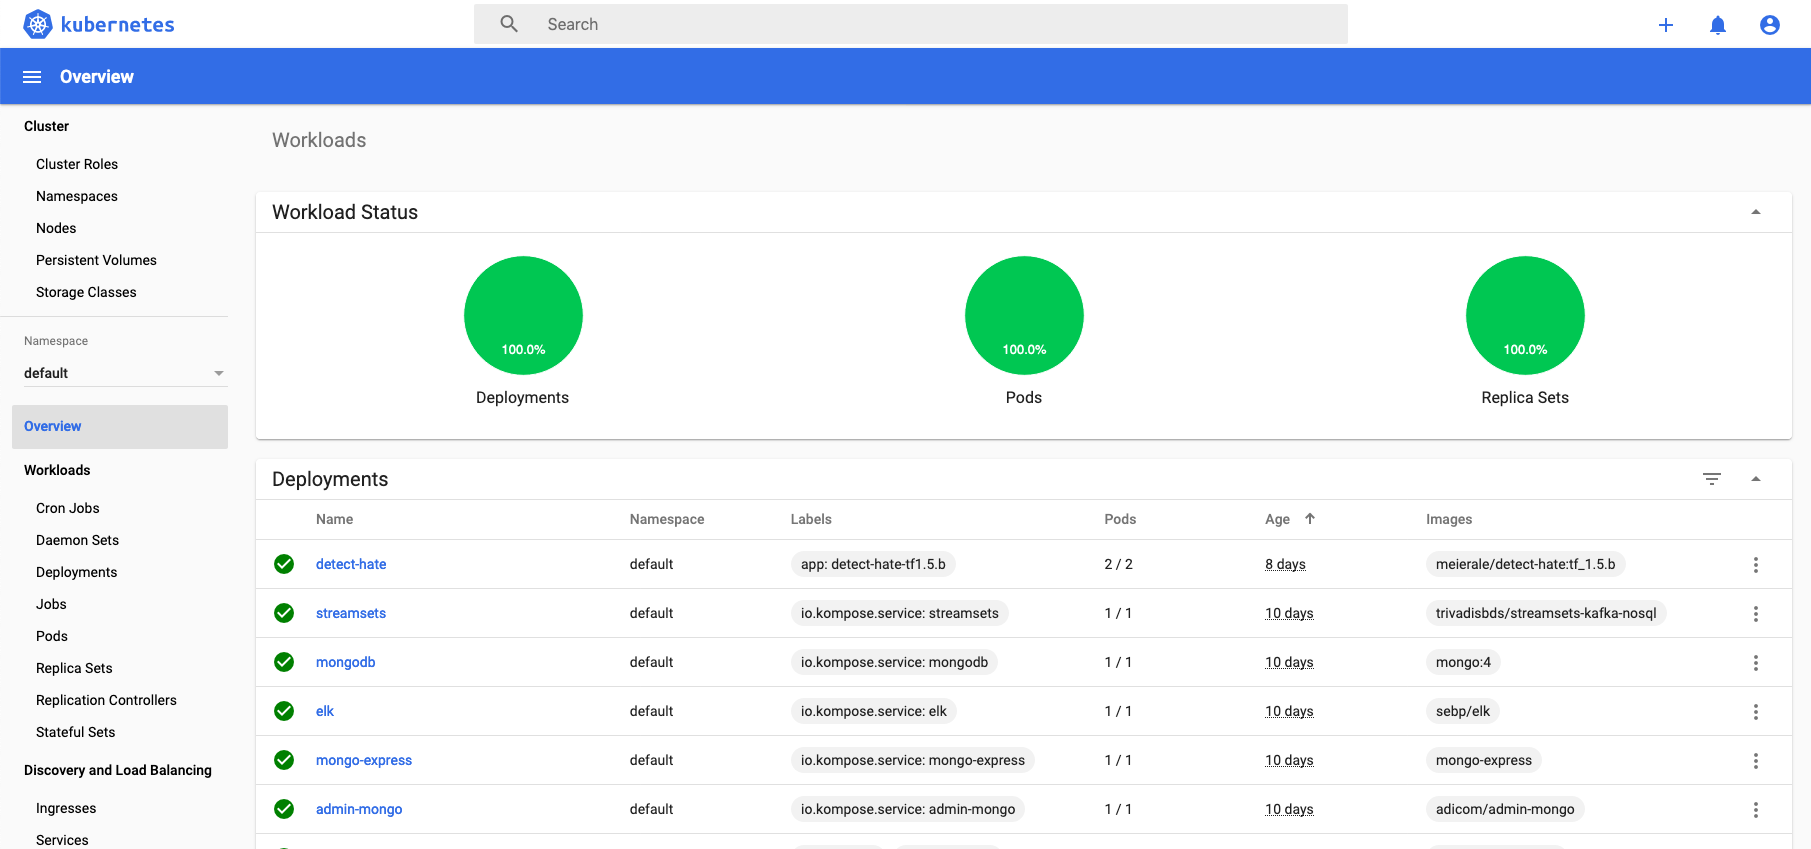
\includegraphics[scale=0.2]{images/kubernetes_overview.png}
	\caption{Kubernetes Dashboard Overview}
	\label{fig:kubernetes_overview}
\end{figure}
 
\textbf{Konvertieren der docker-compose Datei f{\"u}r Kubernetes}

Da Kubernetes einige Unterschiede zu Docker aufweist und somit mit docker-compose.yml nicht umgeben kann, musste die Datei in Kubernetes kompatible Dateien (deployment und service yaml files) konvertiert werden. Hierf{\"u}r gibt es ein Konvertierungstool namens \href{http://kompose.io}{Kompose}. Kompose kann docker-compose Dateien mit einem einfachen Befehl f{\"u}r Kubernetes oder OpenShift umwandeln. Die Software wurde auf dem Master installiert und anschliessend wurde die Datei mit \texttt{kompose convert} konvertiert.

Nach dem Konvertieren der docker-compose Datei wurden Gesamthaft 30 Kubernetes .yaml Dateien erstellt. Zwar ist es m{\"o}glich alles in einer einzigen Datei zu schrieben, dies ist jedoch nicht sinnvoll. Diese Datei w{\"a}re sehr gross, un{\"u}bersichtlich und w{\"u}rde thematisch nicht zusammenh{\"a}ngendes vermischen. Auch im Sinne der Fehlersuche, Wartbarkeit und Erweiterbarkeit ist eine Trennung wichtig. 

Dies zeigt auch, das die Komplexit{\"a}t auf einem Big Data Cluster mit Kubernetes um einiges gr{\"o}sser ist als lokal mit einem Rechner. Wie eingangs erw{\"a}hnt darum auch das Vorgehen zuerst lokal zu entwickeln und sp{\"a}ter auf den Cluster zu wechseln.

Im folgenden wird der Aufbau der einzelnen Kubernetes Dateien wieder anhand der MongoDB aufgef{\"u}hrt. Im Code sind die mongodb-deployment.yaml \ref{lst:kubernetes_deploy.yml},  mongodb-service.yaml \ref{lst:kubernetes_service.yml} und mongodb-volume-persistentvolumeclaim.yaml \ref{lst:kubernetes_persistentvolumeclaim.yml}  Dateien zu sehen.

\begin{lstlisting}[float=h,language=bash,frame=tb,caption={Kubernetes mongodb-deployment.yaml},label=lst:kubernetes_deploy.yml]
apiVersion: extensions/v1beta1
kind: Deployment
metadata:
  annotations:
    kompose.cmd: kompose convert
    kompose.version: 1.17.0 (a74acad)
  creationTimestamp: null
  labels:
    io.kompose.service: mongodb
  name: mongodb
spec:
  replicas: 1
  strategy:
    type: Recreate
  template:
    metadata:
      creationTimestamp: null
      labels:
        io.kompose.service: mongodb
    spec:
      containers:
      - env:
        - name: MONGO_INITDB_DATABASE
          value: sample
        - name: MONGO_INITDB_PASSWORD
          value: admin
        - name: MONGO_INITDB_USERNAME
          value: admin
        image: mongo:4
        name: mongodb
        ports:
        - containerPort: 27017
        resources: {}
        volumeMounts:
        - mountPath: /data/db
          name: mongodb-volume
      restartPolicy: Always
      volumes:
      - name: mongodb-volume
        persistentVolumeClaim:
          claimName: mongodb-volume
status: {}
\end{lstlisting}  

\begin{lstlisting}[float=h,language=bash,frame=tb,caption={Kubernetes mongodb-service.yaml},label=lst:kubernetes_service.yml]
apiVersion: v1
kind: Service
metadata:
  annotations:
    kompose.cmd: kompose convert
    kompose.version: 1.17.0 (a74acad)
  creationTimestamp: null
  labels:
    io.kompose.service: mongodb
  name: mongodb
spec:
  ports:
  - name: "27017"
    port: 27017
    targetPort: 27017
  selector:
    io.kompose.service: mongodb
status:
  loadBalancer: {}
\end{lstlisting} 

\begin{lstlisting}[float=h,language=bash,frame=tb,caption={Kubernetes mongodb-persistentvolumeclaim.yaml},label=lst:kubernetes_persistentvolumeclaim.yml]
apiVersion: v1
kind: Service
metadata:
  annotations:
    kompose.cmd: kompose convert
    kompose.version: 1.17.0 (a74acad)
  creationTimestamp: null
  labels:
    io.kompose.service: mongodb
  name: mongodb
spec:
  ports:
  - name: "27017"
    port: 27017
    targetPort: 27017
  selector:
    io.kompose.service: mongodb
status:
  loadBalancer: {}
\end{lstlisting}

\textbf{Software Konfigurationen}

Analog zur lokalen Anwendung wurde auch die Software Konfigurationen von Kapitel \ref{sec:tool_konfigurieren} auf dem nHex vorgenommen.

Mit dem Befehl \ref{lst:kubernetes_start.yml} lassen sich die Kubernetes deployments und services starten. 

\begin{lstlisting}[float=h,language=bash,frame=tb,caption={Kubernetes start deployments und services},label=lst:kubernetes_start.yml]
$ for f in *.yaml; do echo $f; done
$ for f in *.yaml; do k3s kubectl apply -f $f; done
\end{lstlisting}

\textbf{Import der Pipelines in StreamSets}

Um die Pipelines nicht komplett neu erstellen zu m{\"u}ssen wurden diese von der lokalen Installation inklusiv den Credentials exportiert. StreamSets bietet diesen Export mit oder ohne Credentials an. Anschliessend wurden die vier Pipelines in StreamSets auf dem nHex importiert und getestet. 

\textbf{Kibana Dashbard importieren}

Kibana bietet ebfalls die M{\"o}glich an einzelne Visualisierungen und komplette Dashboards zu exportieren und importieren. Auch hier wurden die erstellten Visualisierungen und das Dashobard lokal exportiert und anschliessend auf dem nHex importiert.





